\chapter{DUNE Physics}
\label{ch:exec-phys}


\textit{
This chapter provides a brief introduction to \dword{dune} physics.  The text below closely follows the presentation in the introductory chapters of Volume~\volnumberphysics{}, 
where many more details may be found.}


\textit{Presented here in summary form are   
(1) the scientific goals and opportunities, 
(2) the key features of the experiment, 
design that enable this program, 
(3) the methodologies we have 
employed to evaluate the capabilities of \dword{dune} to realize 
the science, and
(4) the corresponding results for selected program elements. 
}  

%%%%%%%%%%%%%%%%%%%%%%%%%%%%%%%%%%%%%%%%%%%%%%%%%%%%%%%%%%%%%%
%%%%%%%%%%%%%%%%%%%%%%%%%%%%%%%%%%%%%%%%%%%%%%%%%%%%%%%%%%%%%%

\section{Goals of the DUNE Science Program}
\label{sec:exec-phys-key-goals}

The primary goals and ancillary science program elements listed in the previous 
chapter represent discovery opportunities at the forefront of particle physics and 
astrophysics.  \dword{dune} has been designed to capitalize on these opportunities with 
a unique set of experimental conditions and capabilities.  In this section we 
elaborate on elements of the science program that motivate the operating principles   
and experimental methodologies of \dword{dune}, which are presented in 
Sections~\ref{sec:exec-phys-operatingprinciples} and 
\ref{sec:exec-phys-assm-meth}, respectively.

The \dword{dune} \dword{nd} will have its own physics program, to be described in the \dword{nd} \dword{cdr}, which is in progress as of this writing.


%%%%%%%%%%%%%%%%%%%%%%%%%%%%%%%%%%%%%%%%%%%%%%%%%%%%%%%%%%%%%%
\subsection{Neutrino Oscillations: Masses, Mixing Angles and CP Violation}

Neutrino oscillations imply nonzero neutrino masses and flavor-mixing 
in the leptonic \dword{cc} interactions.  The nonzero neutrino mass is among the most important discoveries in fundamental 
particle physics of the twenty-first century. Understanding the mechanism 
behind nonzero neutrino masses is among the unresolved mysteries that 
drive particle physics today; they remain one of the few unambiguous 
facts that point to the existence of new particles and interactions, 
beyond those that make up the remarkable standard model of 
particle physics.

Almost all neutrino data can be understood within the three-flavor paradigm 
with massive neutrinos,
the simplest extension of the standard model capable of reconciling 
theory with observations.  
It consists of introducing distinct, nonzero, masses for at least two 
neutrinos, while maintaining the remainder of the standard model. Hence, neutrinos 
interact only via the standard model \dword{cc} and \dword{nc}  weak 
interactions. The neutrino mass eigenstates -- defined as $\nu_1,\nu_2, \nu_3$ 
with masses, $m_1, m_2, m_3$, respectively -- are distinct from the neutrino 
\dword{cc} interaction eigenstates, also referred to as the flavor 
eigenstates -- $\nu_e$, $\nu_{\mu}$, $\nu_{\tau}$, labeled according 
to the respective charged-lepton $e,\mu,\tau$ to which they couple in 
the \dword{cc} weak interaction. The flavor eigenstates can be expressed 
as linear combinations of the mass eigenstates: 
the coefficients of the respective linear combinations define a 
unitary $3\times 3$ mixing matrix, the \dword{pmns}
%Pontecorvo-Maki-Nakagawa-Sakata (PMNS)
 matrix, as follows:
\begin{equation}
\left(\begin{array}{c} \nu_e \\ \nu_{\mu} \\ \nu_{\tau} \end{array}\right) = \left(\begin{array}{ccc} U_{e1} & U_{e2} & U_{e3} \\  U_{\mu1} & U_{\mu2} & U_{\mu3}  \\  U_{\tau1} & U_{\tau2} & U_{\tau3}  \end{array}\right) \left(\begin{array}{c} \nu_1 \\ \nu_2 \\ \nu_3 \end{array}\right).
\end{equation}
Nonzero values for at least some of the off-diagonal elements, coupled with nonzero 
differences in the masses of $\nu_1$, $\nu_2$ and $\nu_3$, lead to the phenomenon of 
neutrino oscillations, in which a neutrino -- %necessarily 
produced in a  
flavor eigenstate -- acquires an oscillating (with frequency proportional to 
the differences of the squares of the neutrino masses, $\Delta m^2_{ij}\equiv m_i^2-m_j^2$) 
probability of interacting as a different flavor.


The \dword{pmns} matrix is the leptonic-equivalent of the \dword{ckm} %Cabibbo-Kobayashi-Maskawa (CKM) matrix 
that describes the \dword{cc} interactions of quark mass 
eigenstates. If the neutrinos are Dirac fermions, the \dword{pmns} matrix, 
like the \dword{ckm}, can be unambiguously parameterized with three mixing 
angles and one complex phase.\footnote{Additional nontrivial phases are present 
if neutrinos are Majorana fermions, but these do not affect oscillations at 
an observable level.} By convention~\cite{Tanabashi:2018oca}, the mixing angles 
are denoted $\theta_{12}$, $\theta_{13}$, and $\theta_{23}$, defined as
\begin{eqnarray}
\tan^2\theta_{12} &\equiv& \frac{|U_{e2}|^2}{|U_{e1}|}, \\
\tan^2\theta_{23} &\equiv& \frac{|U_{\mu3}|^2}{|U_{\tau3}|}, \\
\sin^2\theta_{13} &\equiv& |U_{e3}|^2,
\end{eqnarray} 
and the complex phase \deltacp is defined as
\begin{equation}
\deltacp \equiv -{\rm arg}(U_{e3}).
\end{equation}
For values of $\deltacp\neq 0,\pi$, and assuming none of the $U_{\alpha i}$ 
vanish ($\alpha=e,\mu,\tau$, $i=1,2,3$), the neutrino mixing matrix is complex 
and \dword{cp}-invariance is violated in the lepton sector. This, in turn, manifests 
itself as different oscillation probabilities, in vacuum, for neutrinos 
and antineutrinos: $P(\nu_{\alpha}\to\nu_{\beta})\neq 
P(\bar{\nu}_{\alpha}\to\bar{\nu}_{\beta})$, $\alpha,\beta=e,\mu,\tau$, $\alpha\neq\beta$.

The central aim of the world-wide program of %long-baseline 
neutrino experiments past, present and planned, is to explore 
the phenomenology of neutrino oscillations in the context of the 
three-flavor paradigm, and, critically, 
to challenge its validity with measurements at progressively 
finer levels of precision.  The world's neutrino data significantly constrain 
all of the oscillation parameters in the three-flavor paradigm, but 
with precision that varies considerably from one parameter to the next.

Central questions remain open. The neutrino mass ordering -- whether $\nu_3$ is 
the heaviest (``normal'' ordering) or the lightest (``inverted'' ordering) -- is unknown. 
Current data prefer the normal ordering, but the inverted one still 
provides a decent fit to the data. The angle $\theta_{23}$ is known to be 
close to the maximal-mixing value of $\pi/4$, but assuming it is not exactly 
so, the octant 
(whether $\sin^2\theta_{23}<0.5$ [$\theta_{23}<\pi/4$] or 
$\sin^2\theta_{23}>0.5$ [$\theta_{23}>\pi/4$]) is also unknown. 
The value of \deltacp is only poorly constrained. While positive 
values of $\sin\deltacp$ are disfavored, all values between $\pi$ and $2\pi$, 
including the \dword{cp}-conserving values $\deltacp=0,\pi$, are consistent with 
the world's neutrino data.  That the best fit to the world's data 
favors large \dword{cpv} is suggestive, providing further impetus 
for experimental input to resolve this question.
All of these questions can be addressed 
by neutrino oscillation experiments.

Conventional horn-focused beams, where either \numu or \anumu 
is the dominant species (depending on horn current polarity), provide 
access to these questions for experiments at long baselines as in the case 
of \dword{lbnf-dune}.  By virtue 
of the near-maximal value of $\theta_{23}$, oscillations are mainly in the  
mode $\nu_\mu \rightarrow \nu_\tau$.  For realizable baselines, 
this channel is best studied by 
measuring the $\nu_\mu$ disappearance probability as a function of 
neutrino energy rather than through direct observation of $\nu_\tau$ 
appearance.  This is because oscillation maxima occur at energies 
below the threshold for $\tau$-lepton production in $\nu_\tau$ 
\dword{cc} interactions in the detector.
On the other hand, the sub-dominant $\nu_\mu \rightarrow \nu_e$ channel is 
amenable to detailed study through the energy dependence of the
$\nu_e$ and $\bar\nu_e$ appearance probabilities, 
which is directly sensitive (in a rather complex way) to 
multiple \dword{pmns} matrix parameters, as described below.  

Specifically, the oscillation probability of \numu $\rightarrow$ \nue 
through matter in a constant density approximation is,  % Anne 3/9
to first order~\cite{Nunokawa:2007qh}:
%
\begin{eqnarray}
P(\nu_\mu \rightarrow \nu_e) & \simeq & \sin^2 \theta_{23} \sin^2 2 \theta_{13} 
\frac{ \sin^2(\Delta_{31} - aL)}{(\Delta_{31}-aL)^2} \Delta_{31}^2 \nonumber \\
& & + \sin 2 \theta_{23} \sin 2 \theta_{13} \sin 2 \theta_{12} \frac{ \sin(\Delta_{31} - aL)}{(\Delta_{31}-aL)} \Delta_{31} \frac{\sin(aL)}{(aL)} \Delta_{21} \cos (\Delta_{31} + \mdeltacp) \nonumber\\
& & + \cos^2 \theta_{23} \sin^2 2 \theta_{12} \frac {\sin^2(aL)}{(aL)^2} \Delta_{21}^2, 
\label{eqn:appprob}
\end{eqnarray}
where $\Delta_{ij} = \Delta m^2_{ij} L/4E_\nu$, $a = G_FN_e/\sqrt{2}$, $G_F$ is the Fermi constant, $N_e$ is the number density of electrons in the Earth, $L$ is the baseline in km, and $E_\nu$ is the neutrino energy in GeV. 
In the equation above, both \deltacp and $a$ 
switch signs in going from the
$\nu_\mu \to \nu_e$ to the $\bar{\nu}_\mu \to \bar{\nu}_e$ channel; i.e.,
a neutrino-antineutrino asymmetry is introduced both by \dword{cpv} (\deltacp)
and the matter effect ($a$). As is evident from Equation~\ref{eqn:appprob}, 
the matter effect introduces a sensitivity to the sign of $\Delta_{31}$, 
which specifies the neutrino mass ordering.
The origin of the matter effect asymmetry 
is simply the presence of electrons and absence of positrons in the Earth.  
In the few-GeV energy range, the asymmetry from the matter effect increases 
with baseline as the neutrinos
pass through more matter; therefore an experiment with a longer baseline will be
more sensitive to the neutrino mass ordering. For baselines longer than 
$\sim$\SI{1200}\km, the degeneracy between the asymmetries from matter
and \dword{cpv} effects can be resolved~\cite{Bass:2013vcg}.

The electron neutrino appearance probability, $P(\nu_\mu \rightarrow \nu_e)$, 
is plotted in 
Figure~\ref{fig:oscprob} at a baseline of \SI{1300}\km{} as a function of neutrino 
energy for several values of \deltacp. As this figure illustrates, the value 
of \deltacp affects both the amplitude and phase of
the oscillation. The difference in probability amplitude
for different values of \deltacp is larger at higher oscillation nodes, which 
correspond to energies less than 1.5~GeV. Therefore, a broadband experiment, 
capable of measuring not only the rate of \nue appearance but of mapping out the 
spectrum of observed oscillations down to energies of at least 500~MeV, is desirable. 

\begin{figure}
  \centering
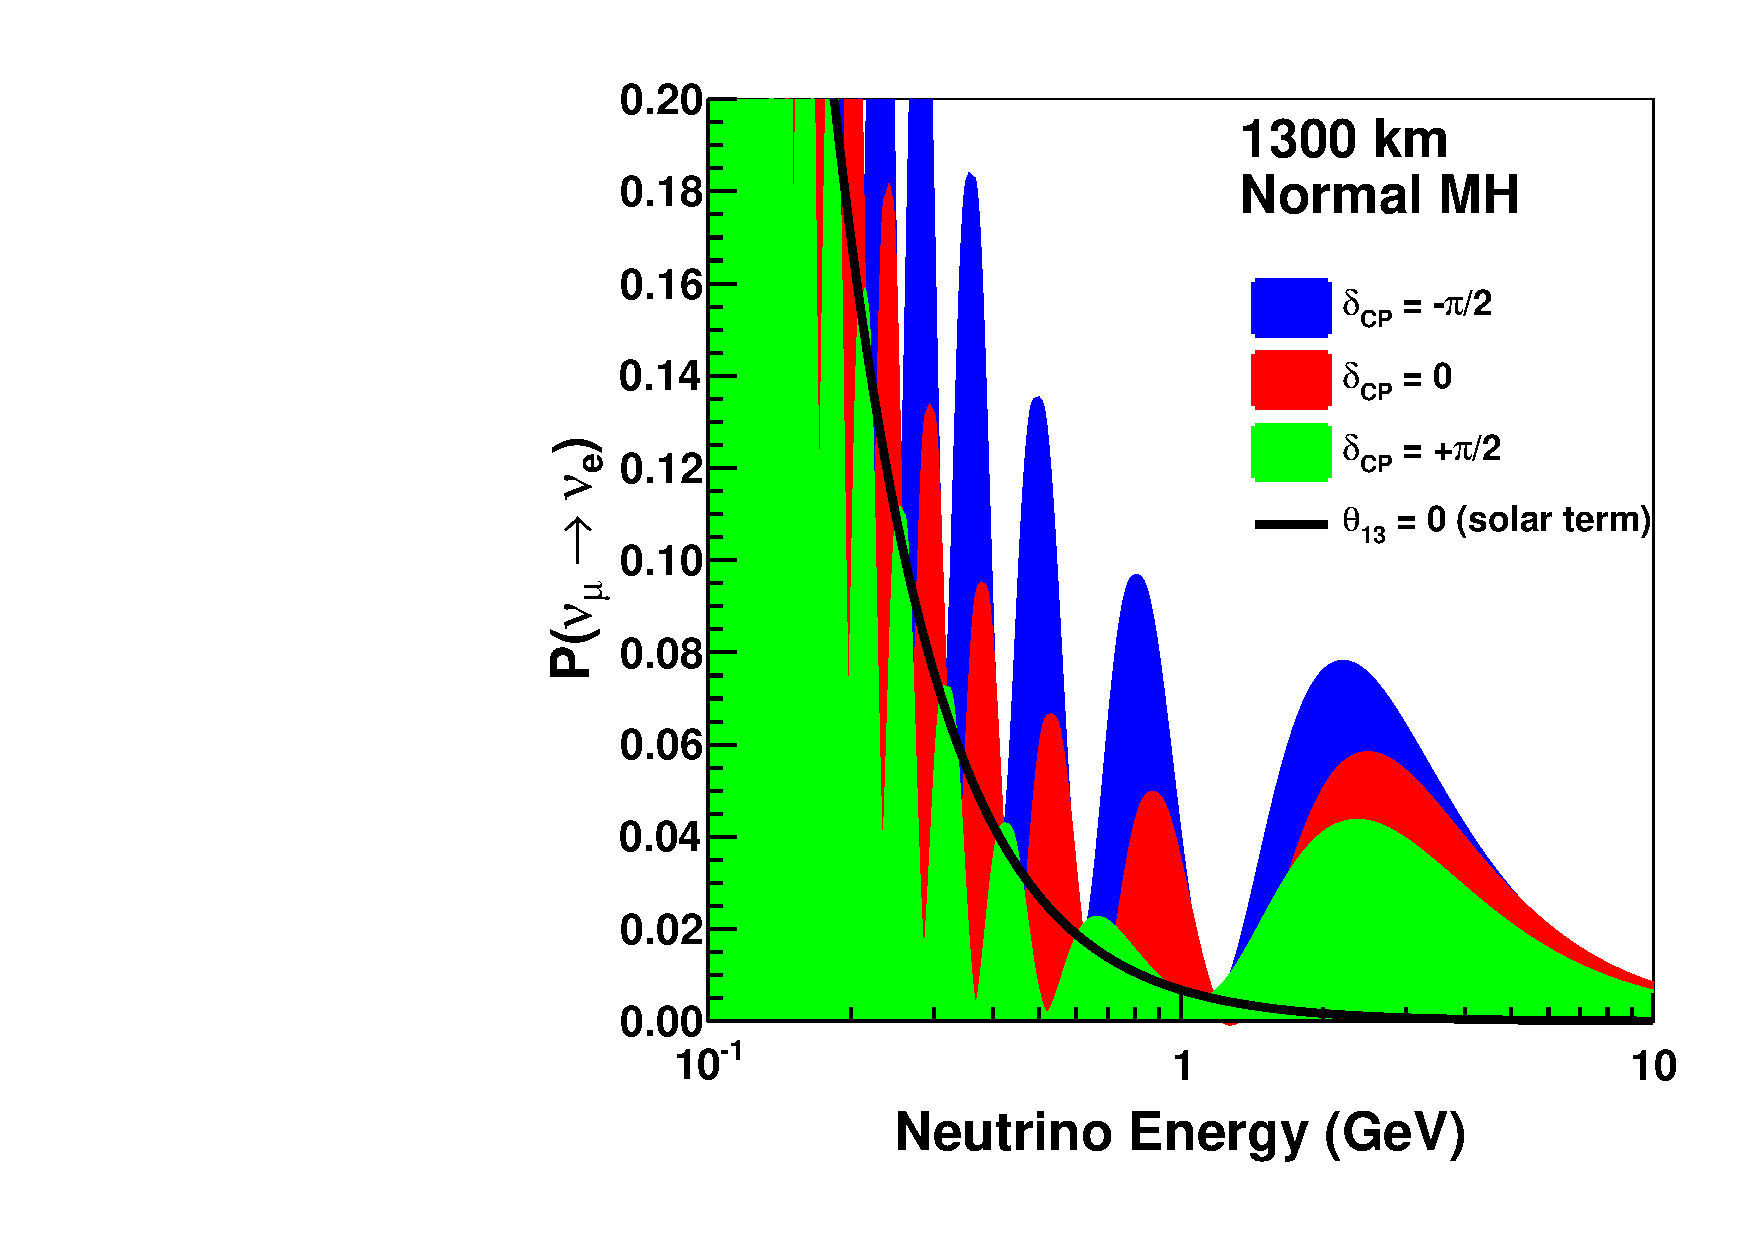
\includegraphics[width=0.45\linewidth]{energy_nu_no.pdf}
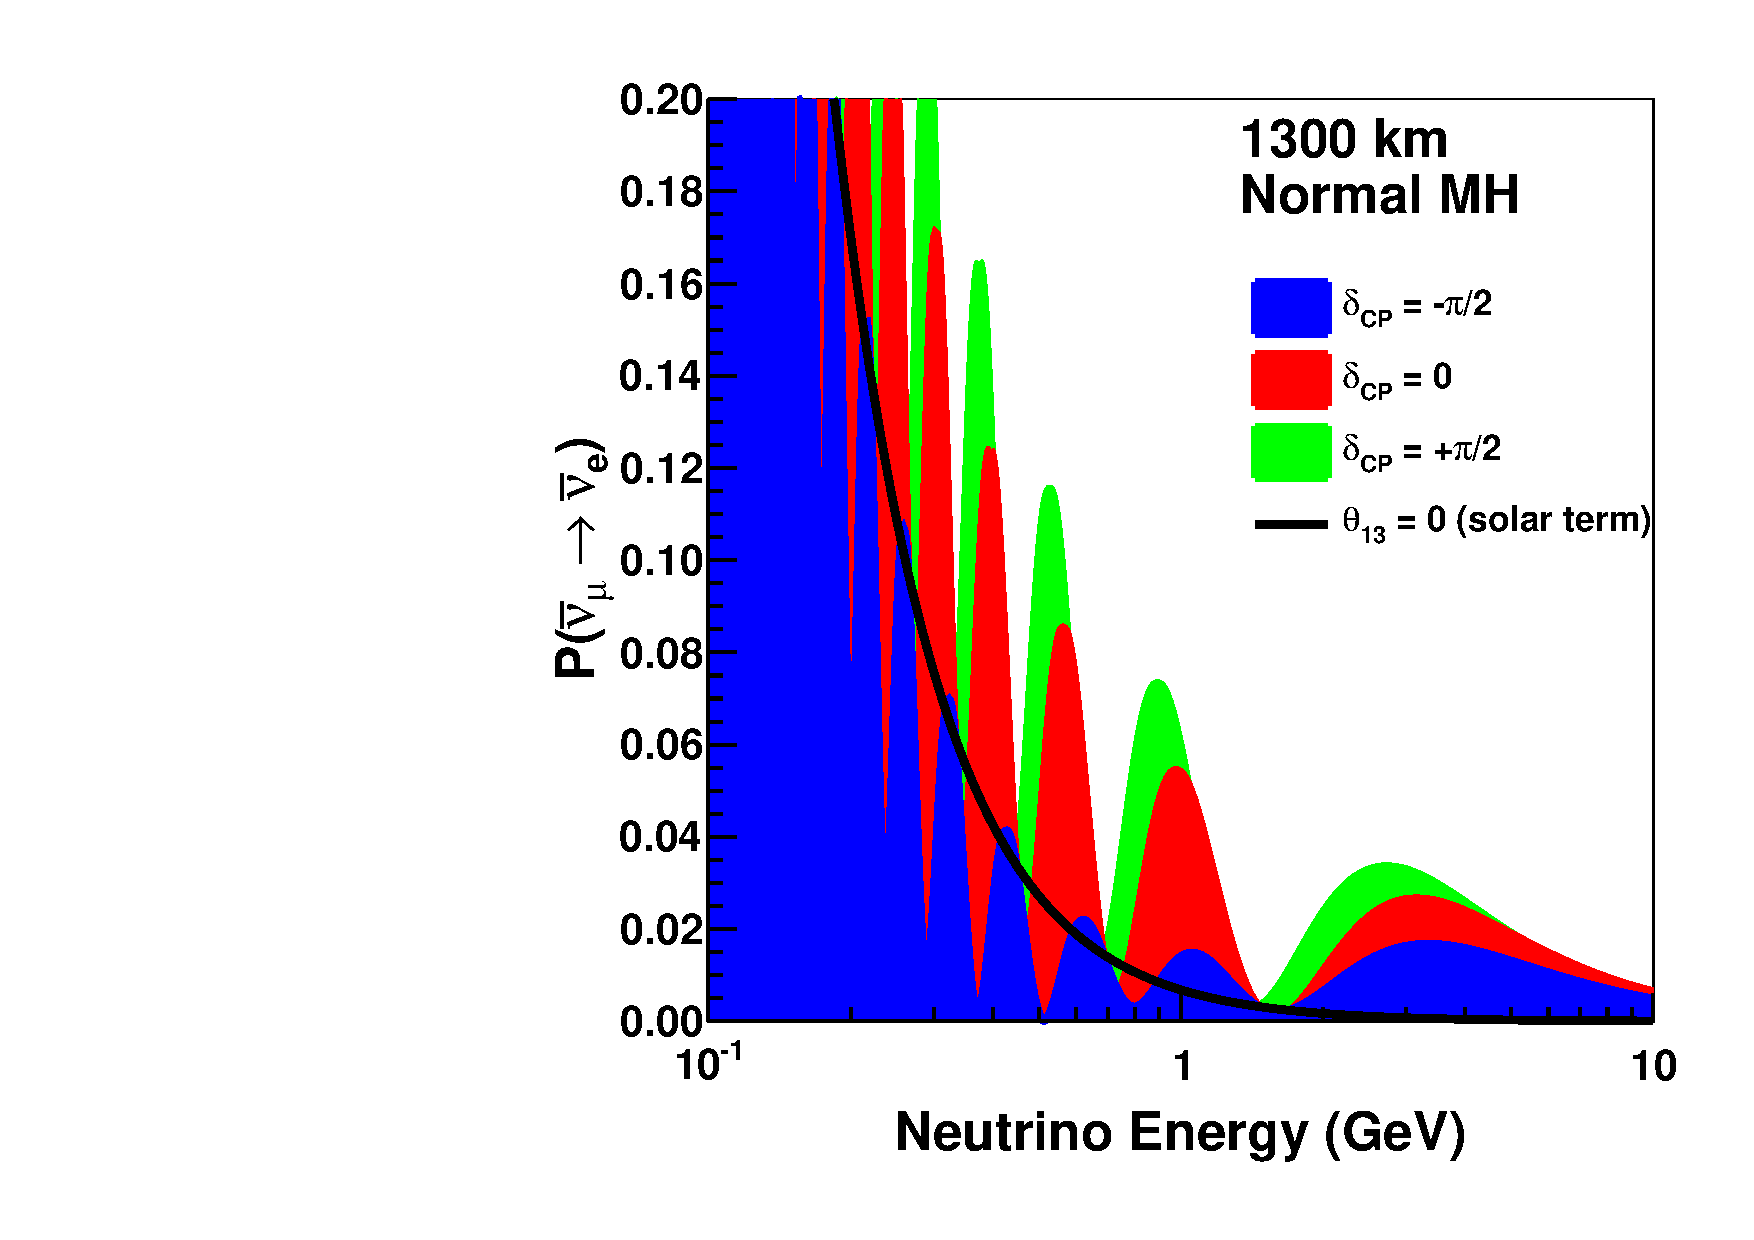
\includegraphics[width=0.45\linewidth]{energy_anu_no.pdf}
  \caption[Appearance probabilities for \nue and \anue at \SI{1300}{\km}]{The appearance probability at a baseline of \SI{1300}\km{},
  as a function of neutrino energy, for \deltacp = $-\pi/2$ (blue), 
  0 (red), and $\pi/2$ (green), for neutrinos (left) and antineutrinos
  (right), for normal ordering. The black line indicates the oscillation
  probability if $\theta_{13}$ were equal to zero. Note that \dword{dune} will be built at a baseline of \SI{1300}{\km}.}
  \label{fig:oscprob}
\end{figure}

\dword{dune} is designed to address the questions articulated above, 
to over-constrain the three-flavor paradigm, 
and to reveal what may potentially lie beyond.  
Even if consistency is found, the precision measurements 
obtained by \dword{dune} will have profound implications. As just one example, 
the discovery of \dword{cpv} in neutrino oscillations would provide 
strong circumstantial evidence for the leptogenesis mechanism as 
the origin of the baryon asymmetry of the universe.  

Going further, the patterns defined by the fermion masses and 
mixing parameters have been the subject of intense theoretical 
activity for the last several decades.  Grand unified theories 
posit that quarks and leptons are different manifestations of the same 
fundamental entities, and thus their masses and mixing parameters 
are related. Different models make different predictions but, 
in order to compare different possibilities, it is important that 
lepton mixing parameters be known as precisely as quark mixing parameters.
To enable equal-footing comparisons between quark and lepton mixing 
it is required 
that the mixing angles be determined at the few percent level 
while $\deltacp$ should be measured at the 10\% level or better.
Measurements with precision at these levels are expected from \dword{dune} 
for the mixing angles $\theta_{23}$ and $\theta_{13}$, 
and the \dword{cp} phase $\deltacp$.   
These measurements will thus open a new era of flavor physics, 
with the potential to offer insight on deep questions on which the 
standard model is essentially silent.

%%%%%%%%%%%%%%%%%%%%%%%%%%%%%%%%%%%%%%%%%%%%%%%%%%%%%%%%%%%%%%
\subsection{Baryon Number Violation}

Are protons %unstable?  
stable? Few questions within elementary 
particle physics can be posed as simply and at the same time 
have implications as immediate.  The 
apparent stability of protons suggests that baryon number 
is conserved in nature, although no known symmetry 
requires it to be so.  Indeed, baryon number conservation is 
implicit in the formulation of the \dword{sm} Lagrangian, and 
thus observation of \dword{bnv} processes such 
as nucleon decay or neutron-antineutron oscillation 
would be evidence for physics beyond the \dword{sm}.
On the other hand, continued non-observation of \dword{bnv} processes will 
demand an answer to what new symmetry is at play that forbids 
them.
 
Especially compelling is that the observation of \dword{bnv} processes 
could be the harbinger for \dwords{gut}, in which strong, weak and 
electromagnetic forces are unified.  Numerous \dword{gut} models 
have been proposed, each with distinct features.  Yet, \dword{bnv} processes 
are expected on general grounds, and it is a feature of many models 
that nucleon decay channels can proceed at experimentally 
accessible rates.  This is illustrated for several key nucleon 
decay channels relevant for \dword{dune} in 
Figure~\ref{fig:theoryexplimitsummary}, along with existing 
experimental limits.

\begin{dunefigure}[Summary of nucleon decay experimental limits and model predictions]{fig:theoryexplimitsummary}{Summary of nucleon decay experimental lifetime limits from past or currently running experiments for several modes, and the model predictions for the lifetimes in the two modes \ptoepizero and \ptoknubar.  The limits shown are 90\% \dword{cl} lower limits on the partial lifetimes, $\tau/B$, where $\tau$ is the total mean life and $B$ is the branching fraction. Updated from~\cite{Babu:2013jba}.}
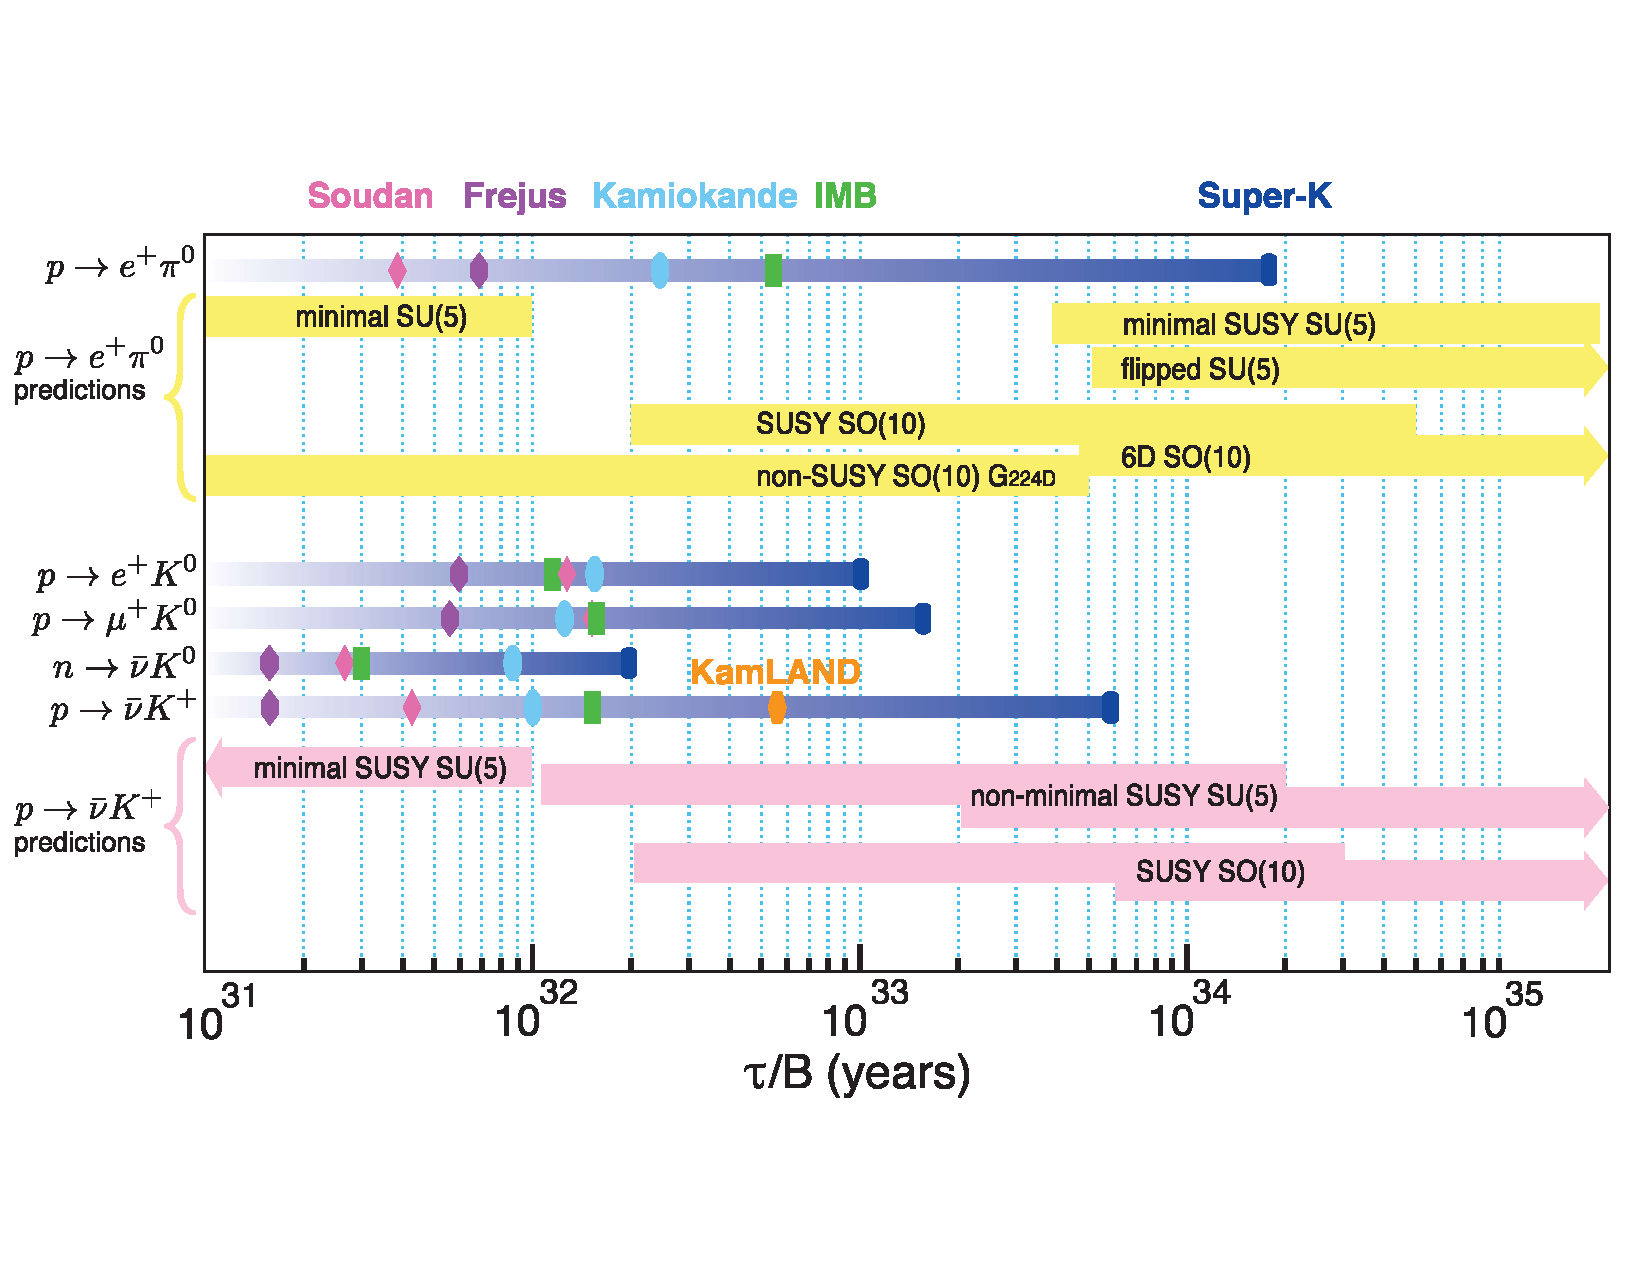
\includegraphics[width=0.9\textwidth]{TheoryExpLimitSummary.pdf}
\end{dunefigure}

Given the scale of energy deposition in the few hundred \si{\MeV} 
to few \si{\GeV} range, 
a detector optimized for neutrino oscillation physics at long 
baselines is naturally well suited for sensitive searches for 
nucleon decay and neutron-antineutron oscillations.
Thanks to the excellent imaging, calorimetric and particle 
identification capabilities of the \dword{lartpc}, 
backgrounds can in principle be reduced below the single event 
level for key nucleon decay channels at exposures where other 
detector technologies are no longer background-free.  On the 
other hand, a challenge presented by an argon-based 
detector is the impact of final-state interactions on 
nucleon decay event reconstruction, which is 
expected to be more severe than for detectors based on water 
or liquid scintillator, for example.  
On balance, however, should nucleon decays occur at rates 
not far beyond current best limits, a handful of candidate 
events could be observed by \dword{dune} in a given decay mode.  
%Even just one or two candidate events would generate considerable 
%excitement.

%%%%%%%%%%%%%%%%%%%%%%%%%%%%%%%%%%%%%%%%%%%%%%%%%%%%%%%%%%%%%%
\subsection{Supernova Neutrino Bursts}

The burst of neutrinos~\cite{Bionta:1987qt,Hirata:1987hu} 
from the celebrated core-collapse supernova 
1987A in the Large Magellanic Cloud, about
\SI{50}{kiloparsecs} (kpc) from Earth, heralded the era of extragalactic neutrino
astronomy.  The few dozen recorded $\bar{\nu}_e$ events
have confirmed the basic physical
picture of core collapse and yielded constraints on a wide range of new
physics~\cite{Schramm:1990pf, Vissani:2014doa}.  

Core-collapse supernovae within a few hundred kpc of Earth --
within our own galaxy and nearby -- are quite rare on a human
timescale.  They are expected once every few decades in the Milky Way
(within about 20~kpc), and with a similar rate in Andromeda, about
700~kpc away.  However, core collapses should be common enough to have
a reasonable chance of occurring during the few-decade long lifetime
of a typical large-scale neutrino detector. % Anne adds per LBNC 12/2:
It is important that at least one module of the\dword{dune} \dword{fd} be online at all times to
observe this unpredictable and spectacular event, if and when it occurs.   
%The rarity of these spectacular events 
The rarity of these events makes it all the more critical for the community to
be prepared to capture every last bit of information from them.

The information in a \dword{snb} available in principle
to be gathered by experimentalists is the \textit{flavor, energy and
  time structure} of a several-tens-of-second-long, all-flavor,
few-tens-of-MeV neutrino burst~\cite{Mirizzi:2015eza, Horiuchi:2017sku}.  Imprinted on
the neutrino spectrum as a function of time is information about the
progenitor, the collapse, the explosion, and the remnant, as well as
information about neutrino parameters and potentially exotic new
physics.  Neutrino energies and flavor content of the burst can be
measured only imperfectly, due to the intrinsic nature of the weak
interactions of neutrinos with matter, as well as due to imperfect
detection resolution in any real detector.  For example, \dword{snb} 
 energies are below \dword{cc} threshold for $\nu_\mu$,
$\nu_\tau$, $\bar{\nu}_\mu$, and $\bar{\nu}_{\tau}$ (collectively
$\nu_x$), which represent two-thirds of the flux; so these flavors are
accessible only via \dword{nc}  interactions, which tend to have
low cross sections and indistinct detector signatures. 
These issues make a
comprehensive unfolding of neutrino flavor, time and energy structure
from the observed interactions a challenging problem.

The core-collapse neutrino signal starts with a short, sharp
\emph{neutronization} (or \emph{break-out}) burst primarily composed of
$\nu_e$. These neutrinos are messengers of the shock front breaking through the neutrinosphere (the surface of neutrino trapping): when this happens, iron is disintegrated, the neutrino scattering cross section drops and the lepton number trapped just below the original neutrinosphere is suddenly released. This quick and intense burst is followed by an
\emph{accretion phase} lasting some hundreds of milliseconds, depending on the progenitor star mass, as matter falls onto the collapsed core and the shock is stalled at the distance of perhaps $\sim 200$ km. The gravitational binding energy of the accreting material is powering the neutrino luminosity during this stage. The later
\emph{cooling phase} over $\sim$10~seconds represents the main part of
the signal, over which the proto-neutron star sheds its trapped energy.  

The flavor content and spectra of the neutrinos emitted from the neutrinosphere change
throughout these phases, and the supernova's evolution can
be followed with the neutrino signal. 
Some fairly generic features of these emitted neutrino fluxes are
illustrated in Figure~\ref{params}.

\begin{dunefigure}[Expected time-dependent neutrino burst 
characteristics for a core-collapse 
supernova]{params}{Expected
  time-dependent signal for a specific flux model for an
  electron-capture supernova~\cite{Huedepohl:2009wh} at 10~kpc.  No oscillations are assumed. Note that $\nu_x$  refers to $\nu_\mu$,
$\nu_\tau$, $\bar{\nu}_\mu$, and $\bar{\nu}_{\tau}$ collectively. The
  top plot shows the luminosity as a function of time ($\nu_x$ is the sum of all, the second plot
  shows average neutrino energy, and the third plot shows the $\alpha$
  (pinching) parameter.  The vertical dashed line at 0.02 seconds indicates
  the time of core bounce, and the vertical lines indicate different
  eras in the supernova evolution.  The leftmost time interval
  indicates the infall period.  The next interval, from core bounce to
  50~ms, is the neutronization burst era, in which the flux is
  composed primarily of $\nu_e$.  The next period, from 50 to 200~ms,
  is the accretion period. The final era, from 0.2 to 9~seconds, is
  the proto-neutron-star cooling period.  The general features are
  qualitatively similar for most core-collapse supernovae.}
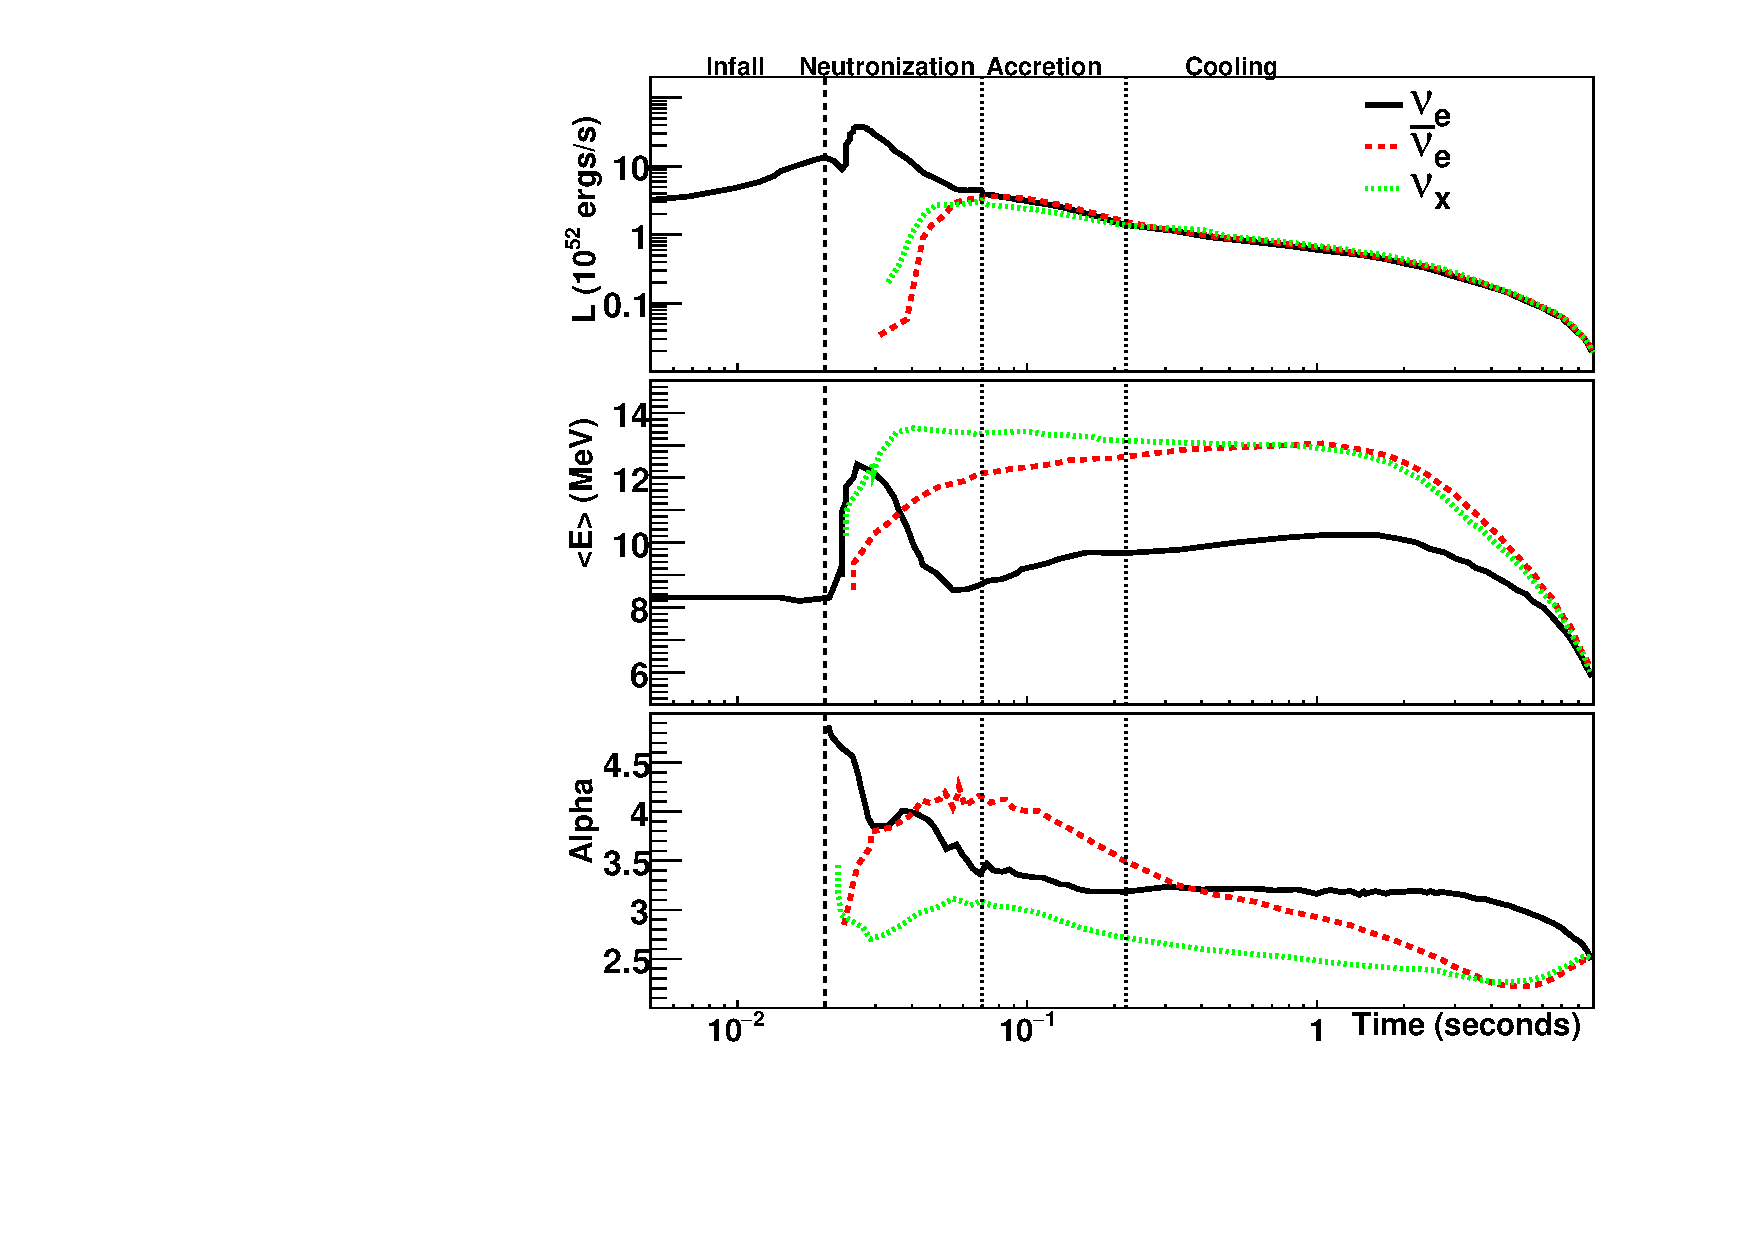
\includegraphics[width=0.9\textwidth]{garching_paramonly.pdf}
\end{dunefigure}

In the world's current supernova neutrino flavor sensitivity
portfolio~\cite{Scholberg:2012id, Mirizzi:2015eza}, the sensitivity 
is primarily to electron antineutrino flavor, via inverse beta decay.  
There is only minor sensitivity to the $\nu_e$
component of the flux, which carries with it particularly interesting 
information content of the burst (e.g., neutronization burst neutrinos
are created primarily as $\nu_e$).  While there is some $\nu_e$
sensitivity in existing and other planned detectors via elastic 
scattering on electrons and via subdominant channels on nuclei, 
statistics are relatively small,
and it can be difficult to disentangle the flavor content.  It is 
in this respect that an experiment with an argon target such as \dword{dune} 
will be especially valuable, since the dominant process in 
this case is $\nu_e$ \dword{cc} scattering.


%%%%%%%%%%%%%%%%%%%%%%%%%%%%%%%%%%%%%%%%%%%%%%%%%
\subsection{Additional Beyond Standard Model Physics Signatures}

The capabilities that enable access to the physics program described 
in the previous sections open a myriad of opportunities to search for 
evidence of physics beyond the standard model.  Below we list the 
identified opportunities that we have investigated.  
Projected sensitivities are shown later in this chapter for only 
a few of these opportunities; we refer the reader to  
Volume~\volnumberphysics{}, \voltitlephysics{}, for a more complete demonstration of 
the potential impact of \dword{dune}'s searches for \dword{bsm} phenomena,  
which can justifiably be considered as prominent ancillary 
elements of the \dword{dune} science program.  At the same time, it is 
important to note that new physics may appear in ways that have 
not yet been considered: history has repeatedly shown that nature 
can reward new experimental approaches and sensitive detectors 
with the appearance of entirely unanticipated phenomena.

Opportunities in \dword{bsm} physics that have been considered 
as elements of the \dword{dune} science program include:

\textit{Search for active-sterile neutrino mixing:} \dword{dune} is sensitive over a broad range of potential sterile neutrino mass splittings by looking for disappearance of \dword{cc} and \dword{nc}  interactions over the long distance separating the \dword{nd} and \dword{fd}, as well as over the short baseline of the \dword{nd}. With a longer baseline, a more intense beam, and a high-resolution large-mass \dword{fd}, compared to previous experiments, \dword{dune} provides a unique opportunity to improve significantly on the sensitivities of the existing probes, and greatly enhance the ability to map the extended parameter space if a sterile neutrino is discovered.

\textit{Searches for non-unitarity of the \dword{pmns} matrix:} Deviation from 
unitarity of the $3 \times 3$ \dword{pmns} matrix due to extra heavy 
neutrino states may be observable. 
Parameters characterizing the degree 
of non-unitarity can
become sizable as the masses of the new states decrease.

\textit{Searches for \dwords{nsi}:} %non-standard neutrino interactions:} Non-standard neutrino interactions, 
\Dwords{nsi} affecting neutrino propagation through the Earth can significantly modify the data to be collected by \dword{dune} as long as the new physics parameters are large enough.  If the \dword{dune} data are consistent with standard oscillations for three massive neutrinos, interaction effects of order 0.1 $G_{F}$ can be ruled out at \dword{dune}.

\textit{Searches for violation of Lorentz or \dword{cpt} symmetry:}  \dword{dune} can improve the present limits on Lorentz and \dword{cpt} violation in the neutrino sector by several orders of magnitude, contributing an important experimental test of these fundamental assumptions underlying quantum field theory.

\textit{Studies of neutrino trident production:}  
Interactions of neutrinos with the Coulomb field of a 
nucleus can lead to final states with a lepton-pair 
accompanying the lepton from the neutrino interaction 
vertex. 
With a predicted annual rate of over 100 dimuon 
neutrino trident interactions at the \dword{nd}, \dword{dune} will be 
able to measure deviations from the \dword{sm} rates and test 
the presence of new gauge symmetries.

\textit{Search for \dword{ldm}:}  The lack of evidence for \dword{wimp} dark matter 
candidates from direct detection and LHC experiments has resulted in a reconsideration of the \dword{wimp} paradigm, and has revitalized the effort to search for light dark matter candidates 
of around a GeV or below in mass. High-flux neutrino beam experiments, such as \dword{dune}, have been shown to provide coverage of \dword{dm}+mediator parameter space that cannot be covered by either direct detection or collider experiments. \dword{dm} particles can be detected in the \dword{nd} through \dword{nc}-like interactions either with electrons or nucleons in the detector material and enable \dword{dune}'s search for \dword{ldm} to be competitive and complementary to other experiments.

\textit{Search for \dword{bdm}:} Using its large \dword{fd}, \dword{dune} will be able to search for  \dword{bdm}. In these models there are several dark matter particles with different masses and
properties concerning their interactions with \dword{sm} particles. \dword{dune} will search for such particles 
as generally produced anywhere in the cosmos or specifically through annihilation 
in the core of the sun, allowing competitive results for both production scenarios

\textit{Search for Heavy Neutral Leptons (HNLs):} HNLs in the context of the $\nu$MSM model with 
masses less than 2 GeV can be produced in the beam-dump of the proton beam to generated the 
\dword{dune} neutrino beam. The \dword{nd} data can be used to search for HNL decays, and competitive
results with other present and proposed facilities can be obtained.

\begin{comment}  From anne per LBNC 12/2
%%%%%%%%%%%%%%%%%%%%%%%%%%%%%%%%%%%%%%%%%%%%%%%%%%%%
\section{General LBNF/DUNE Operating Principles}
\label{sec:exec-phys-operatingprinciples}

World-wide scientific and technical planning for the
ambitious next-generation deep underground long-baseline
neutrino oscillation experiment that \dword{lbnf-dune} now represents
has been under way for more than a decade.  Much
development preceded the formation of the \dword{dune} science
collaboration in 2015 (see, for example,
Refs.~\cite{Adams:2013qkq} and \cite{LAGUNA-LBNO-deliv}).

Extensive study and discussion within the community on 
how best to address the scientific challenges described 
in the preceding section 
have led to the principal features of the \dword{lbnf-dune}
configuration:

\textit{High-intensity conventional wide-band
  $\nu_\mu$ beam}	The current generation of long-baseline neutrino experiments
	have benefited from narrow-band beam characteristics 
	associated with off-axis detector deployment. The principal 
	advantage is a low background rate in both \nue appearance 
	and \numu disappearance channels from misidentified \dword{nc}  interactions of high energy neutrinos.  
	However, this advantage comes at a cost of flux and 
	spectral information relative to an on-axis detector 
    configuration~\cite{Adams:2013qkq,Agarwalla:2014tca}.
    The \dword{dune} concept
    builds on the notion that a highly-performant detector
    technology (see below) 
    with excellent neutrino energy reconstruction
    and background rejection capabilities can
    optimize sensitivity and cost with an on-axis exposure to
    an intense conventional (magnetic horn-focused) beam.

\textit{Far detector site selection for long baseline}
    As discussed in the preceding section, 
    the \SI{1300}{\km} baseline offered by locating the \dword{dune} \dword{fd}
    at the Sanford Underground Research Facility in Lead, 
    South Dakota is well-optimized for the neutrino oscillation 
    physics goals of the program~\cite{Bass:2013vcg}.

\textit{Deep underground location for far detector modules}
    Early studies (see, {\sl e.g.}, Ref.~\cite{homestake:depth}) 
    demonstrated that to realize the non-accelerator based elements
    of the \dword{dune} science program, a deep underground \dword{fd}
    location is required.  These studies also indicate that the 
    4850 Level of Sanford Lab provides sufficient attenuation of 
    cosmic rays in the rock above, conclusions that have been 
    supported by more recent studies (see,
    {\sl e.g.}, Refs.~\cite{bib:docdb3384,bib:docdb1752}).


\textit{\lartpc technology for far detector modules}
    Combining intrinsic scalability with high-performance event 
    imaging, calorimetry and particle identification capabilities, 
    the concept of large \dword{lartpc} detectors was developed 
    for the broad underground science program of \dword{dune}.  This design choice integrates well with the
    other basic design elements described above.
    For example, the
    excellent neutrino energy reconstruction capability
    of \dwords{lartpc} 
    is especially important for the long-baseline program with a 
    wide-band neutrino beam.
    Additionally, the choice of \dword{lartpc} technology provides 
    valuable complementarity to other 
    existing and planned detectors pursuing many
    of the same goals.  As an example of this complementarity,
    the sensitivity of \dword{dune} to the \nue component of supernova 
    neutrino flux, prevalent in the neutronization phase of the 
    explosion, provides distinct information relative to that 
    provided by water or organic scintillator-based detectors in 
    which \anue interactions dominate.  
%\end{itemize}

The scientific basis for the above foundational experimental
design choices has been examined and validated through extensive
review, undertaken at all stages of \dword{dune} development.
Recent experimental and theoretical developments have only
strengthened the scientific case for \dword{dune} and its
basic configuration.  The technical underpinnings for
these choices have also been strengthened over time through a world-wide
program of R\&D and engineering development, as described in a suite
of \dword{lbnf-dune} project documents including this \dword{tdr}, as
well as in sources describing independent experiments and development
activities.
\end{comment}  From anne per LBNC 12/2

%%%%%%%%%%%%%%%%%%%%%%%%%%%%%%%%%%%%%%%%%%%%%%%%%%%%%%%%%%%%%%                                   
\section{Summary of Assumptions and Methods Employed}
\label{sec:exec-phys-assm-meth}

Scientific capabilities are determined assuming \dword{dune}
is configured according to the general parameters described above.
Further assumptions regarding the neutrino beam and detector 
systems, and their deployment, are stated here in
Sections~\ref{sec:exec-phys-assm-meth-beamdetector} and
\ref{sec:exec-phys-assm-meth-deployment}. 

Determination of experimental sensitivities relies on the
modeling of the underlying physics and background processes,
as well as the detector response, including calibration and
event reconstruction performance and the utilization of data
analysis techniques and tools.
A brief discussion of the strategies employed is given below
in Section~\ref{sec:exec-phys-assm-meth-simreco}. 

\subsection{Beam and Detector}
\label{sec:exec-phys-assm-meth-beamdetector}

Physics sensitivities are based on 
the optimized design of a \SI{1.2}{MW} neutrino beam and
corresponding protons-on-target per year assumed to
be 1.1 $\times 10^{21}$ POT.  These numbers assume a combined
uptime and efficiency of the \fnal accelerator complex and the
\dword{lbnf} beamline of 56\%.\footnote{This projection, from which one  
year of \dword{lbnf} beam operations can be expressed as \SI{1.7e7}{seconds}, 
is based on extensive 
experience with intense neutrino beams at Fermilab, and in particular 
the \dword{numi} beam line, which incorporates elements like those in the  
proposed \dword{lbnf} beamline design and faces similar operating conditions.} 

For the neutrino oscillation physics program, it is assumed that
equal exposures (time-integrated beam power times fiducial mass) are obtained with both horn current polarities,
and therefore with the corresponding mix of primarily \numu
and \anumu data samples.

It is assumed that the \dword{dune} \dword{fd} will include some
combination of the different \nominalmodsize fiducial volume
implementations (single or dual-phase) of the \dword{lartpc} concept
for which technical designs have been developed.                                                     
For much of the science program it is expected that the
capabilities of the two proposed \dword{fd} module 
implementations will be comparable.  As a result of the
current state of reconstruction and analysis software development
(see Section~\ref{sec:exec-phys-assm-meth-simreco}), the
physics sensitivity studies reported in this \dword{tdr} are based on
the single-phase \dword{lartpc} implementation,
documented in full in Volume~\volnumbersp{}. %\voltitlesp{}.

It is also assumed that validation of the \dword{dune} \dword{fd} 
designs will come from data and operational experience acquired 
with the large-scale ProtoDUNE detectors staged at CERN, 
including single-particle studies of data obtained 
in test-beam running.  

The \dword{nd} for \dword{dune} has been under active development,
and a \dword{cdr} is in preparation.
Correspondingly, the descriptions utilized in this \dword{tdr}
are consistent with this level of development.  

\subsection{Deployment Scenario}
\label{sec:exec-phys-assm-meth-deployment}

Where presented as a function of calendar year,
sensitivities are calculated with the following
assumed deployment plan, which is based on a
technically limited schedule:
\begin{itemize}
    \item Start of beam run: Two \dword{fd} module %FD 
    volumes for total fiducial mass of 20 kt, 1.2 MW beam
    \item After one year: Add one \dword{fd} module  volume for total fiducial mass of 30 kt
    \item After three years: Add one \dword{fd} module  volume for total fiducial mass of \fdfiducialmass
    \item After six years: Upgrade to 2.4 MW beam
\end{itemize}


\subsection{Simulation, Reconstruction and Data Analysis Tools}
\label{sec:exec-phys-assm-meth-simreco}

The development of algorithms and software infrastructure needed
to carry out physics sensitivity studies has been an active 
effort within \dword{dune} and the associated scientific community.  
Significant progress has been made: event reconstruction 
codes can be run on fully simulated neutrino interaction events 
in \dword{dune} \dword{fd} modules; the \dword{dune} computing infrastructure 
allows high-statistics production runs; and end-user interfaces 
are functioning.  Robust end-to-end analyses not previously
possible have now been performed and are being 
reported in this document.

For some aspects -- for example, beamline modeling
and GeV-scale neutrino interaction simulations --
well-developed and validated (with data) software packages have
been available throughout much of \dword{dune}'s design phase.
For others, corresponding tools did not exist and needed to be
either developed from scratch or adapted with substantial
modifications from other experimental programs.  Concurrent
with these development efforts, interim descriptions such
as parametric detector response modeling, necessarily simple
but based on reasonable extrapolation from experience and
dedicated studies, were employed to assess physics capabilities.
Even for the case of the better-developed tools -- again, neutrino 
interaction modeling is a good example -- significant incremental
improvements have been made as data from neutrino experiments
and other sources have become available and as theoretical
understandings have advanced.

As a result of the rapid pace of development as well as 
practical considerations including human 
resource availability, different levels
of rigor have been applied in the evaluation of physics 
capabilities for different elements of the program.  
The strategy adopted for
this TDR has been to hold the primary elements of the program
to the highest standard of rigor, involving direct analysis
of fully simulated data, utilizing actual event reconstruction
codes and analysis tools that could be applied to real data
from \dword{dune} \dword{fd} modules.  For other elements of the
program, sensitivities utilize realistic beam and
physics simulations, but employ parametric detector
response models in place of full reconstruction.

The implementation of this strategy comes with caveats
and clarifications that are discussed in the corresponding
chapters of Volume~\volnumberphysics{}.   
Some of these are mentioned here.
\begin{itemize}
\item In the case of the long-baseline oscillation physics
      program, this approach requires a combination of the 
      fully end-to-end analysis of simulated \dword{fd} data
      with the concurrent analysis of simulated data from
      \dword{nd} systems to capture in a realistic way 
      the level of 
      control over systematic errors.  Given the 
      current state of development \dword{dune} \dword{nd} design and 
      corresponding analysis tools,  it has been necessary to 
      employ parametric detector response modeling for near 
      detector components. 

\item In the case of the nucleon decay searches, 
      reconstruction and analysis tools dedicated toward
      addressing the particular challenges presented are 
      not as well developed as in the case of the 
      beam-based oscillation physics program. Effort is 
      ongoing to improve the performance of these tools. 

\item The \dword{snb}  program relies on 
reconstruction of event signatures from \dword{lartpc} signals 
generated by low-energy (MeV-scale) particles (electrons 
and de-excitation gammas).  Full simulation and reconstruction 
is used for some studies, such as for those demonstrating 
the supernova pointing capability of \dword{dune}.  
For other studies, a modified strategy is employed in order 
to efficiently explore model space:  reconstruction metrics 
(resolution smearing matrices, for example) are derived 
from analysis of fully simulated and reconstructed low-energy 
particles and events in the \dword{fd}, and applied to 
understand mean detector response over a range of signal predictions.

\item For scientific program elements where
      analysis of fully reconstructed simulated data has 
      not yet been performed, the parametric response models 
      used for the analyses presented here have
      been well characterized with dedicated studies
      and incorporation of results from other experiments.
      The demonstration of sensitivities for the long-baseline
      oscillation physics program (with full reconstruction) 
      that are comparable to those
      previously obtained based on parametric response
      validates this approach.
\end{itemize}


%%%%%%%%%%%%%%%%%%%%%%%%%%%%%%%%%%%%%%%%%%%%%%%%%%%%%%%%%%%%%%                                   
\section{Selected Results from Sensitivity Studies}
\label{sec:exec-phys-sensitiv-results}

In this section, selected sensitivity projections from the 
central elements of the \dword{dune} science program are presented.  
This selection is intended to convey just the headlines from 
what is an extensive and diverse program of frontier science.

%%%%%%%%%%%%%%%%%%%%%%%%%%%%%%%%%%%%%%%%%%%%%%%%%%%%%%%%%%%%%%
\subsection{\dshort{cpv} in the Neutrino 
Sector and Precise Oscillation Parameter Measurements}
\label{sec:es:phys:cpv}

The key strength of the \dword{dune} design concept is its ability to 
robustly measure the oscillation patterns of \numu and \anumu 
over a range of energies spanning the first and second 
oscillation maxima. 

This is accomplished by a coordinated analysis of the 
reconstructed \numu, \anumu, \nue, and \anue energy spectra 
in near and far detectors, 
incorporating data collected with forward (neutrino-dominated) 
and reverse (antineutrino-dominated) horn current polarities.  

The statistical power of \dword{dune} relative to the current 
generation of long-baseline oscillation experiments 
is a result of many factors including  
(1) on-axis operations, (2) the \dword{lbnf} beam power, 
(3) long baseline and correspondingly high energy 
oscillation maxima and strong separation of 
normal and inverted neutrino mass ordering scenarios, 
(4) detector mass, and (5) event 
reconstruction and selection capabilities. 
Tables~\ref{tab:execsumm-apprates} and 
\ref{tab:execsumm-disrates} 
give the expected event 
yields for the appearance (\nue and \anue) and 
and disappearance (\numu and \anumu) channels, respectively, 
after seven years of operation, assuming $\mdeltacp = 0$ and
\dword{nufit}~\cite{Esteban:2018azc,nufitweb} 
values for other parameters.  Figures~\ref{fig:appspectra} and~\ref{fig:disspectra} show the corresponding distributions in reconstructed neutrino energy.
%
\begin{dunetable}
[\nue and \anue appearance yields]
{lrr}
{tab:execsumm-apprates}
{\nue and \anue appearance yields: Integrated yield of selected $\nu_e$ \dword{cc}-like events between 0.5 and 8.0~GeV assuming \num{3.5}-year (staged) exposures in the neutrino-beam and antineutrino-beam modes.  The signal yields are shown for both normal mass ordering (NO) and inverted mass ordering (IO), and all the background yields assume normal mass ordering.  All the yields assume $\mdeltacp = 0$, and \dword{nufit}~\cite{Esteban:2018azc,nufitweb} 
values for other parameters.}
& \multicolumn{2}{c}{Expected Events (3.5 years staged per mode)} \\ \toprowrule
 & $\nu$ mode & $\bar{\nu}$ mode  \\
 \colhline 
 \nue Signal NO (IO) & 1092 (497) & 76 (36) \\
 \anue Signal NO (IO) & 18 (31)   & 224 (470) \\
  \colhline
 Total Signal NO (IO) & 1110 (528) & 300 (506) \\
  \colhline 
 Beam $\nu_{e}+\bar{\nu}_{e}$ \dword{cc} background & 190 & 117 \\
 \dword{nc} background & 81  & 38\\
 $\nu_{\tau}+\bar{\nu}_{\tau}$ \dword{cc} background & 32 & 20 \\
 $\nu_{\mu}+\bar{\nu}_{\mu}$ \dword{cc} background & 14 & 5 \\
  \colhline
 Total background & 317 & 180\\
 
\end{dunetable}


\begin{dunetable}
[\numu and \anumu disappearance yields]
{lrr}
{tab:execsumm-disrates}
{\numu and \anumu disappearance yields: Integrated yield of selected $\nu_{\mu}$ \dword{cc}-like events between 0.5 and 8.0~GeV assuming a \num{3.5}-year (staged) exposure in the neutrino-beam mode and antineutrino-beam mode.  The yields are shown for normal mass ordering and $\mdeltacp = 0$.}
& Expected Events (3.5 years staged)\\ \toprowrule
  $\nu$ mode & \\
 \colhline 
 \numu Signal & 6200 \\
 \colhline %\toprowrule
  \anumu \dword{cc} background & 389 \\
 \dword{nc} background & 200 \\
 $\nu_{\tau}+\bar{\nu}_{\tau}$ \dword{cc} background & 46 \\
 $\nu_e+\bar{\nu}_e$ \dword{cc} background & 8 \\
 \toprowrule
% \toprowrule
 $\bar{\nu}$ mode  & \\
\colhline % \toprowrule
 \anumu Signal & 2303 \\
\colhline % \toprowrule
  \numu \dword{cc} background & 1129 \\
 \dword{nc} background & 101 \\
 $\nu_{\tau}+\bar{\nu}_{\tau}$ \dword{cc} background & 27 \\
 $\nu_e+\bar{\nu}_e$ \dword{cc} background & 2 \\
\end{dunetable}

\begin{dunefigure}[\nue and \anue appearance spectra]{fig:appspectra}
{\nue and \anue appearance spectra: Reconstructed energy distribution of selected \nue \dword{cc}-like events assuming 3.5 years (staged) running in the neutrino-beam mode (left) and antineutrino-beam mode (right), for a total of seven years (staged) exposure.  The plots assume normal mass ordering and include curves for $\mdeltacp = -\pi/2, 0$, and $\pi/2$.}
 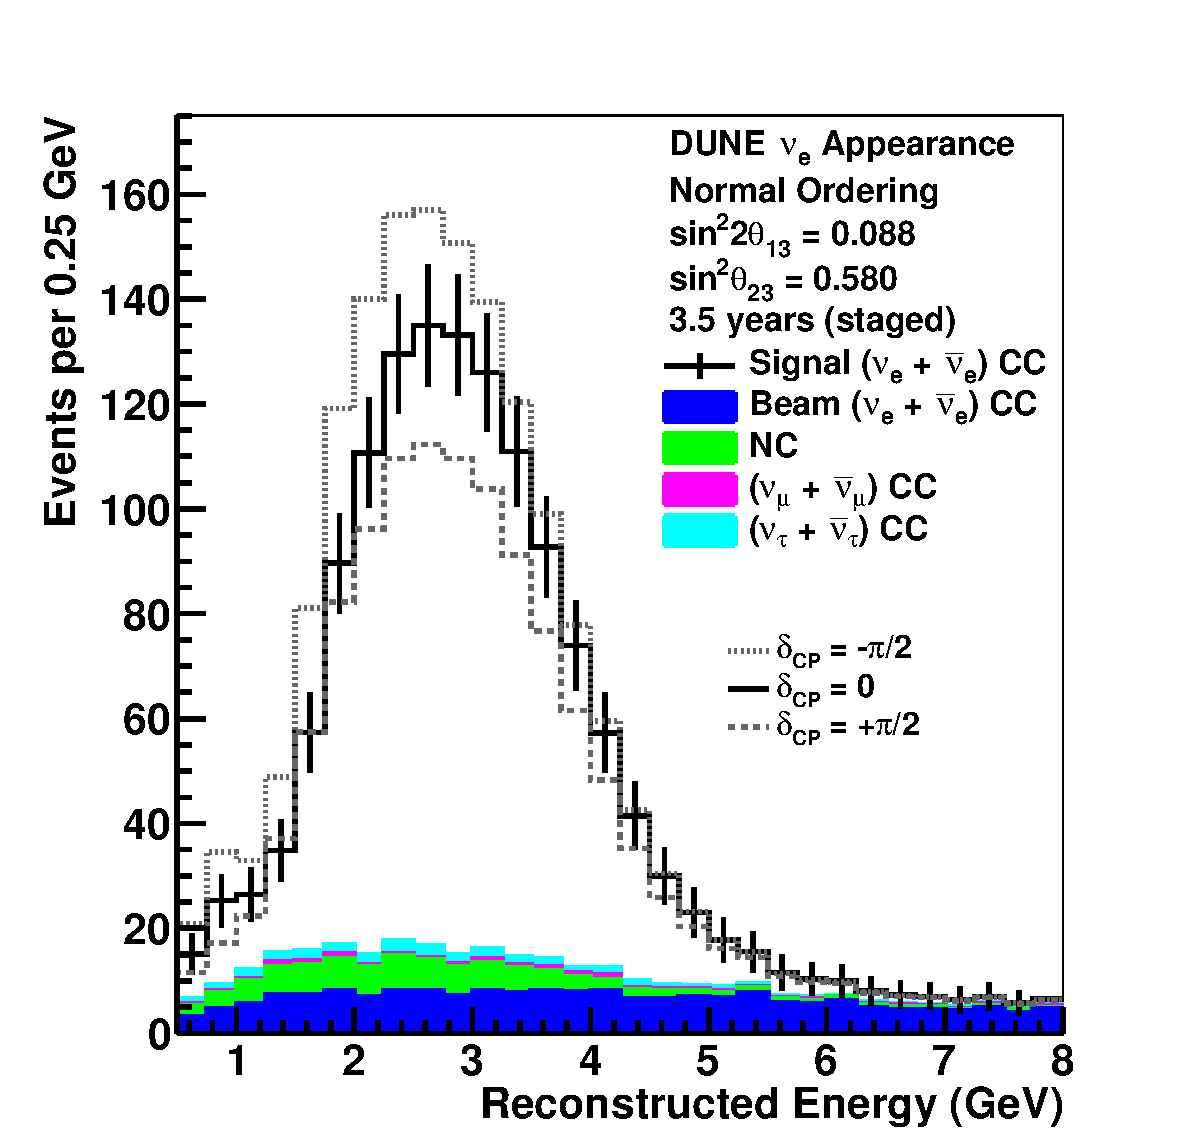
\includegraphics[width=0.49\textwidth]{spec_app_nu_varydcp.pdf}
 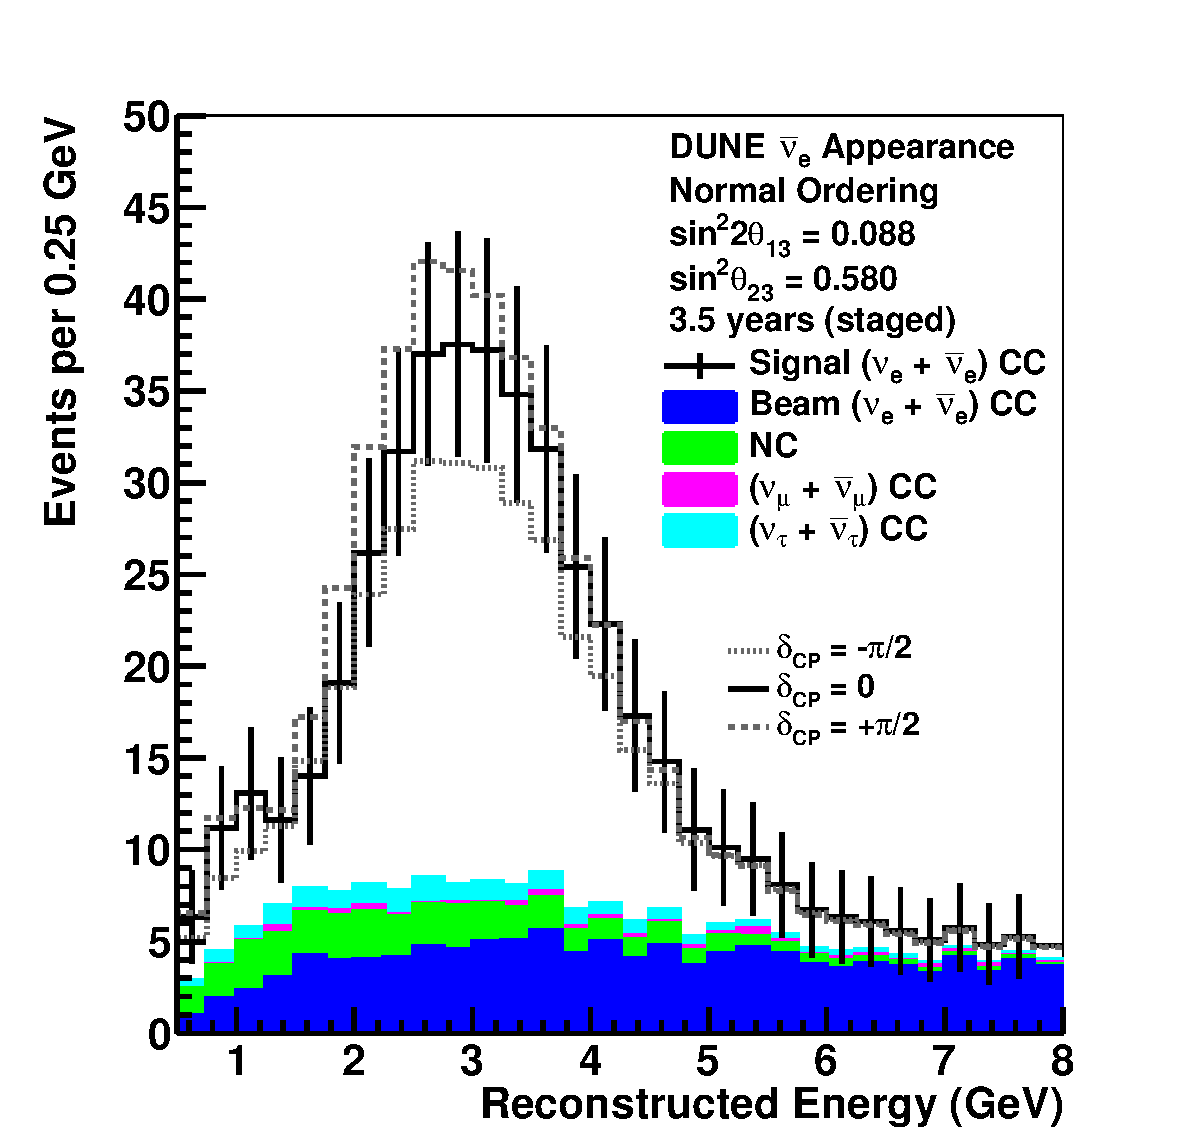
\includegraphics[width=0.49\textwidth]{spec_app_anu_varydcp.pdf}
\end{dunefigure}



\begin{dunefigure}[\numu and \anumu disappearance spectra]{fig:disspectra}
{\numu and \anumu disappearance spectra: Reconstructed energy distribution of selected $\nu_{\mu}$ \dword{cc}-like events assuming 3.5 years (staged) running in the neutrino-beam mode (left) and antineutrino-beam mode (right), for a total of seven years (staged) exposure. The plots assume normal mass ordering.}
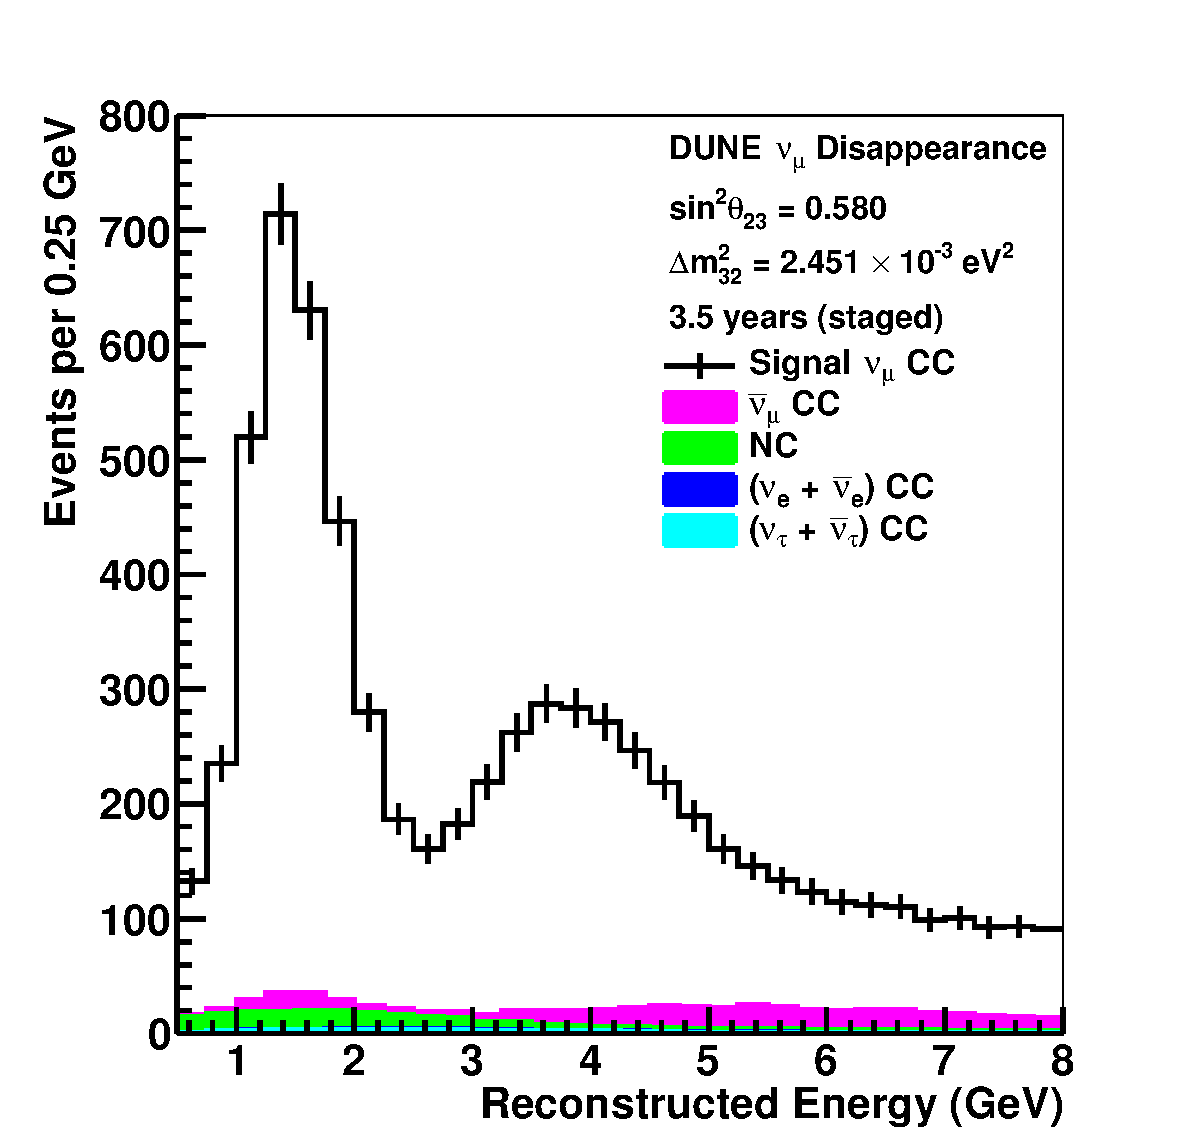
\includegraphics[width=0.49\textwidth]{spec_dis_nu.pdf}
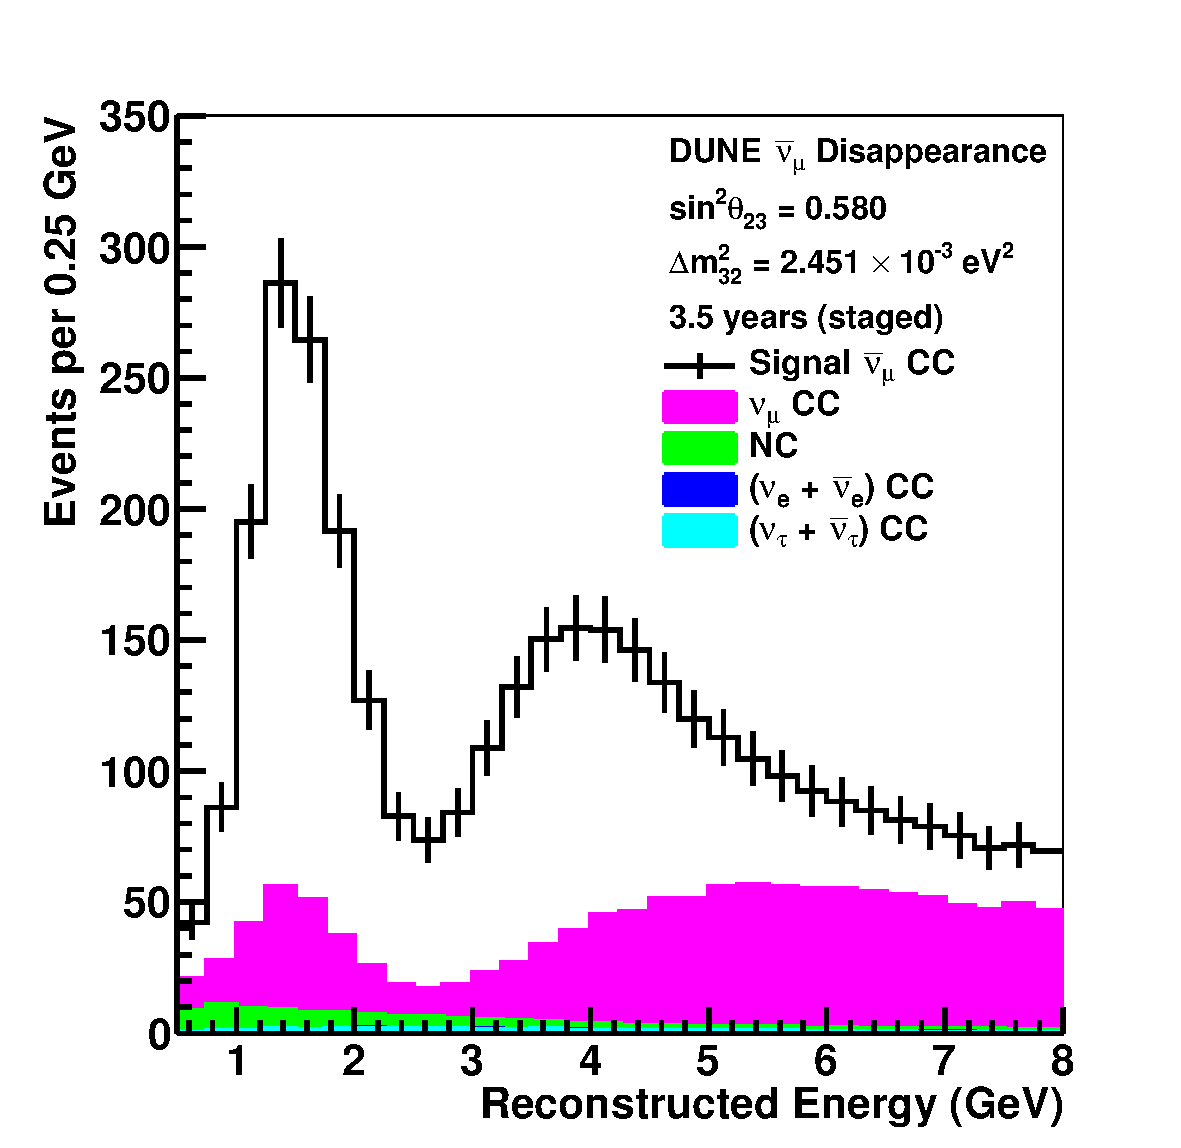
\includegraphics[width=0.49\textwidth]{spec_dis_anu.pdf}
\end{dunefigure}

Experimental sensitivities were evaluated 
based on the methodologies described in the preceding section, 
including incorporation of \dword{nd} simulations 
and uncertainties from all known sources of systematic error.  
%A concrete description of the treatment of systematic errors and 
%the crucial role of the near detector is not possible here given 
%the summary nature of the chapters in this volume.  
%However, it is important to note that 
%Considerable attention and sophistication has been applied to these aspects of the DUNE experimental sensitivity determination, and is documented at length in Volume~\volnumberphysics{}, \voltitlephysics{}.
Considerable attention and sophistication 
has been applied to the treatment of systematic errors and the crucial role of the \dword{nd}, 
both of which are documented in 
Volume~\volnumberphysics{}, \voltitlephysics{}.



A summary of representative sensitivity milestones for neutrino 
mass ordering and \dword{cpv} discovery, as well as precision on 
\deltacp and \sinstt{13} is given in 
Table~\ref{tab:milestones_execsumm-es}.  
The ultimate level of 
precision that can be obtained on oscillation parameters 
highlights the point that \dword{dune} will provide crucial input for  
flavor physics:  Patterns required by particular symmetries 
underlying fermion masses and mixing angles may appear.  The 
unitarity of the neutrino mixing matrix can be tested directly 
through comparisons of \sinstt{13} with the value obtained from 
reactor experiments.  In conjunction with \sinstt{13} and 
other parameters, the precise value of \deltacp can  
constrain models of leptogenesis that are leading 
candidates for explanation of the baryon asymmetry of the universe.

\begin{dunetable}[Projected DUNE oscillation physics milestones]
{lcc}
{tab:milestones_execsumm-es}
{Exposure in years, assuming true normal ordering and equal 
running in neutrino and antineutrino mode, required to reach 
selected physics milestones in the nominal analysis, using the 
NuFIT 4.0~\cite{Esteban:2018azc,nufitweb} best-fit values for the oscillation parameters. As 
discussed in \physchlbl, there are 
significant variations in sensitivity with the value of
\sinst{23}, so the exact values quoted here 
(using \sinst{23} = 0.580) are strongly dependent on that choice. 
The staging scenario presented in
Section~\ref{sec:exec-phys-assm-meth-deployment} is assumed. Exposures 
are rounded to the nearest year.}
 Physics Milestone & Exposure (staged years) \\
 5$\sigma$ Mass Ordering & 1 \\
 \phantom{xxx}(\deltacp = -$\pi/2$) & \\ \colhline
 5$\sigma$ Mass Ordering & 2 \\
 \phantom{xxx}(100\% of \deltacp values) & \\ \colhline
 3$\sigma$ \dshort{cpv} & 3 \\
 \phantom{xxx}(\deltacp = -$\pi/2$) & \\ \colhline
 3$\sigma$ \dshort{cpv} & 5 \\
 \phantom{xxx}(50\% of \deltacp values) & \\ \colhline
 5$\sigma$ \dshort{cpv} & 7 \\
 \phantom{xxx}(\deltacp = $-\pi/2$) & \\ \colhline
 5$\sigma$ \dshort{cpv} & 10 \\
 \phantom{xxx}(50\% of \deltacp values) & \\ \colhline
 3$\sigma$ \dshort{cpv} & 13 \\
 \phantom{xxx}(75\% of \deltacp values) & \\ \colhline
 \deltacp Resolution of 10 degrees & 8 \\
 \phantom{xxx}(\deltacp = 0) & \\ \colhline
 \deltacp Resolution of 20 degrees & 12 \\
 \phantom{xxx}(\deltacp = -$\pi/2$) & \\ \colhline
 \sinstt{13} Resolution of 0.004 & 15 \\ 
\end{dunetable}

The milestones presented in Table~\ref{tab:milestones_execsumm-es} 
form a coarse snapshot of the \dword{dune} program in oscillation physics, 
demonstrating the prospects for important results throughout 
the lifetime of the experiment.  More detail on the 
sensitivities for the individual program elements
is presented in the sections below.

\subsubsection{Discovery Potential for \dshort{cpv} and Neutrino 
Mass Ordering}

Figure~\ref{fig:cpv_staging_execsum} 
illustrates \dword{dune}'s ability to distinguish 
the value of the \dword{cp} phase \deltacp from \dword{cp}-conserving 
values (0 or $\pi$) as a function of time in calendar year.  
These projections incorporate a sophisticated treatment of systematic 
error, as described in detail in \physchlbl.  
%Strong e
Evidence ($>3\sigma$) for \dword{cpv} is obtained for 
favorable values (half of the phase space) of \deltacp after five 
years of running, leading to a $>5\sigma$ %determination 
observation after ten years.

\begin{dunefigure}[Significance of the DUNE determination of 
CP-violation]{fig:cpv_staging_execsum}
{Significance of the DUNE determination of CP-violation (i.e.: \deltacp 
$\neq 0$ or $\pi$) for the case when \deltacp=$-\pi/2$, and for 50\% and 
75\% of possible true \deltacp values, as a function of time in calendar 
years. True normal ordering is assumed. The width of the band shows the 
impact of applying an external constraint on \sinstt{13}.}
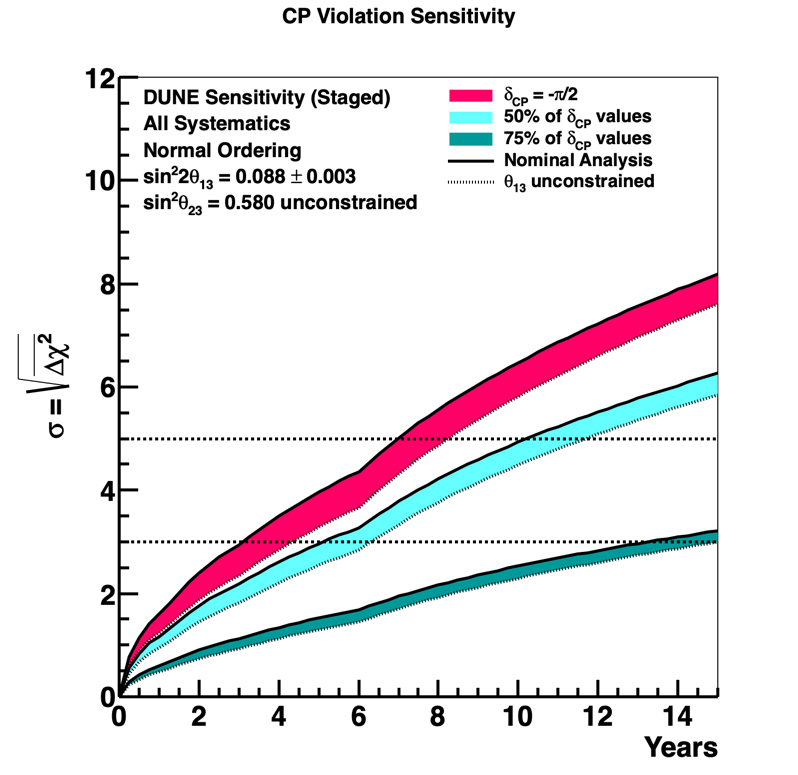
\includegraphics[width=0.75\linewidth]{cpv_exp_staging_varyconstr_nh_2019_v4.png}
\end{dunefigure}

Figure~\ref{fig:mh_staging} shows the significance
with which the neutrino mass ordering can be determined for 100\% of \deltacp values, and when $\deltacp=-\pi/2$, as a function of exposure in years. The width of the bands show the impact of applying an external constraint on \sinstt{13}. As \dword{dune} will be able to establish the neutrino mass ordering at the 5$\sigma$ level for 100\% of \deltacp values after 2-3 years, this plot extends only to seven years.

\begin{figure}[h!]
    \centering
	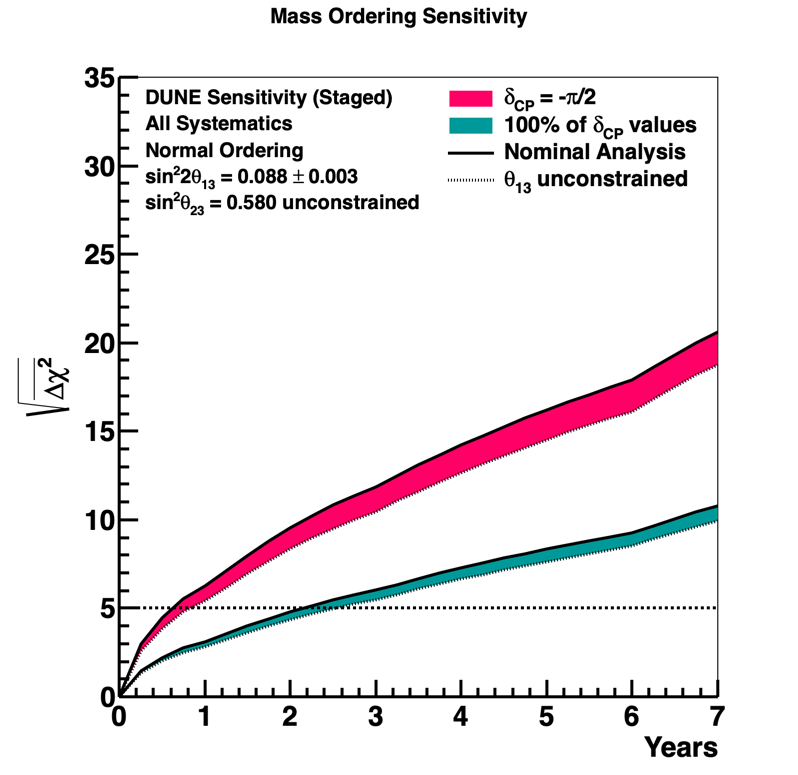
\includegraphics[width=0.75\linewidth]{mh_exp_staging_varyconstr_nh_2019_v4.png}	
	\caption[Significance of the DUNE neutrino mass ordering determination, as a function of time]{Significance of the DUNE determination of the neutrino mass ordering for the case when \deltacp=$-\pi/2$, and for 100\% of possible true \deltacp values, as a function of time in calendar years. True normal ordering is assumed. The width of the band shows the impact of applying an external constraint on \sinstt{13}.}
    \label{fig:mh_staging}
\end{figure}

\subsubsection{Precision Measurement of Mass and Mixing Parameters}

In addition to the discovery potential for neutrino mass ordering and \dword{cpv}, 
\dword{dune} will improve the precision on key parameters that govern neutrino oscillations, including: \deltacp, $\sin^22\theta_{13}$, \dm{31}, $\sin^2\theta_{23}$ and the octant of $\theta_{23}$. 

Figure~\ref{fig:dcpresvdcp} shows the resolution, in degrees, of \dword{dune}'s measurement of \deltacp, as a function of the true value of \deltacp. The resolution of this measurement is significantly better near \dword{cp}-conserving values of \deltacp, compared to maximally \dword{cp}-violating values. For fifteen years of exposure, resolutions between five and fifteen degrees are possible, depending on the true value of \deltacp. 

\begin{figure}[h!]
    \centering
		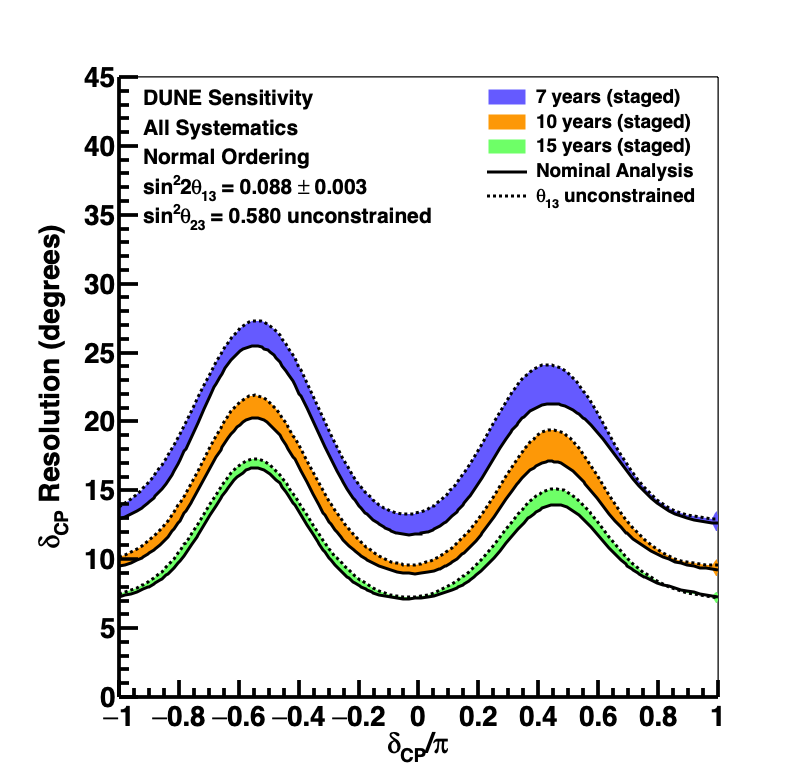
\includegraphics[width=0.75\linewidth]{dcpresvdcp_smooth_v4.png}
	\caption[Resolution for the DUNE measurement of \deltacp as a function of \deltacp]
	{Resolution in degrees for the DUNE measurement of \deltacp, as a function of the true value of \deltacp, for seven (blue), ten (orange), and fifteen (green) years of exposure. True normal ordering is assumed. The width of the band shows the impact of applying an external constraint on \sinstt{13}.}
    \label{fig:dcpresvdcp}
\end{figure}

Figures \ref{fig:appres_exp} and  \ref{fig:disres_exp} show the resolution of \dword{dune}'s measurements of \deltacp and \sinstt{13} and of \sinstt{23} and $\Delta m^{2}_{32}$, respectively, as a function of exposure in kt-MW-years. As seen in Figure~\ref{fig:dcpresvdcp}, the \deltacp resolution varies significantly with the true value of \deltacp, but for favorable values, resolutions near five degrees are possible for large exposure. The \dword{dune} measurement of \sinstt{13} approaches the precision of reactor experiments for high exposure, allowing a comparison between the two results, which is of interest as a test of the unitarity of the \dword{pmns} matrix. 

\begin{figure}[h!]
    \centering
    \begin{tabular}{cc}
		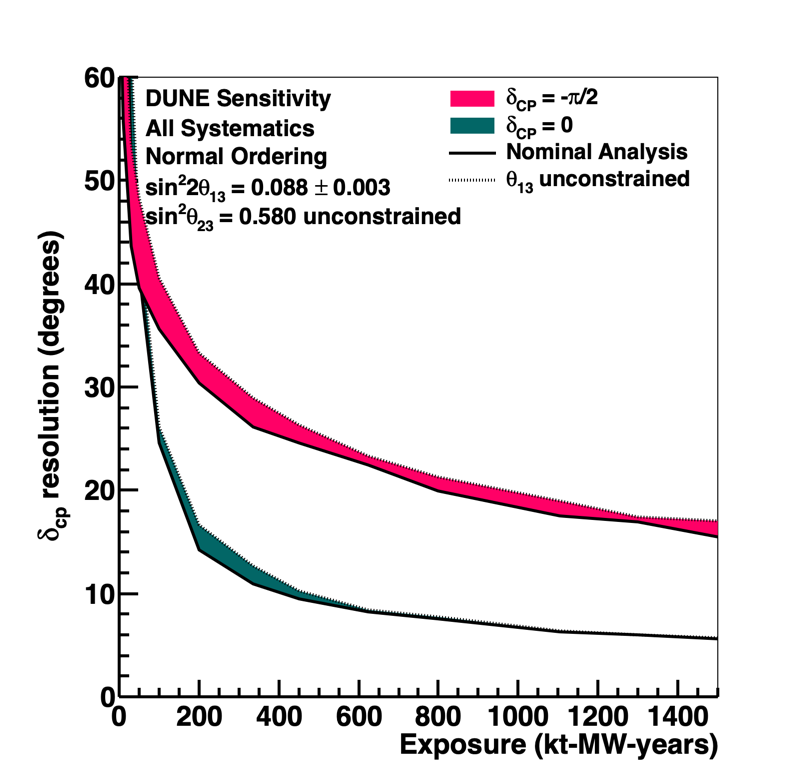
\includegraphics[width=0.475\linewidth]{dcpres_exp_varyconstr_nh_2019_v4.png} &
		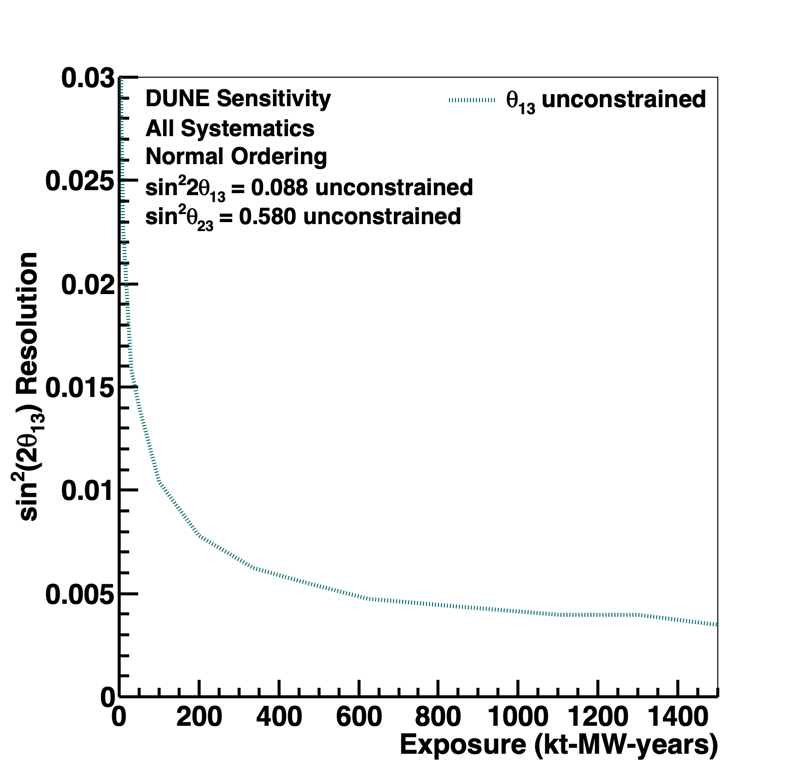
\includegraphics[width=0.475\linewidth]{th13res_exp_varyconstr_nh_2019_v4.png} 
	\end{tabular}  
	\caption[Resolution of DUNE measurements of \deltacp and \sinstt{13}, as a function of exposure]{Resolution of DUNE measurements of \deltacp (left) and \sinstt{13} (right), as a function of exposure in kt-MW-years. As seen in Figure~\ref{fig:dcpresvdcp}, the \deltacp resolution has a significant dependence on the true value of \deltacp, so curves for $\deltacp=-\pi/2$ (red) and $\deltacp=0$ (green) are shown. The width of the band shows the impact of applying an external constraint on \sinstt{13}. For the \sinstt{13} resolution, an external constraint does not make sense, so only the unconstrained curve is shown.}
    \label{fig:appres_exp}
\end{figure}

\begin{figure}[h!]
    \centering
    \begin{tabular}{cc}
		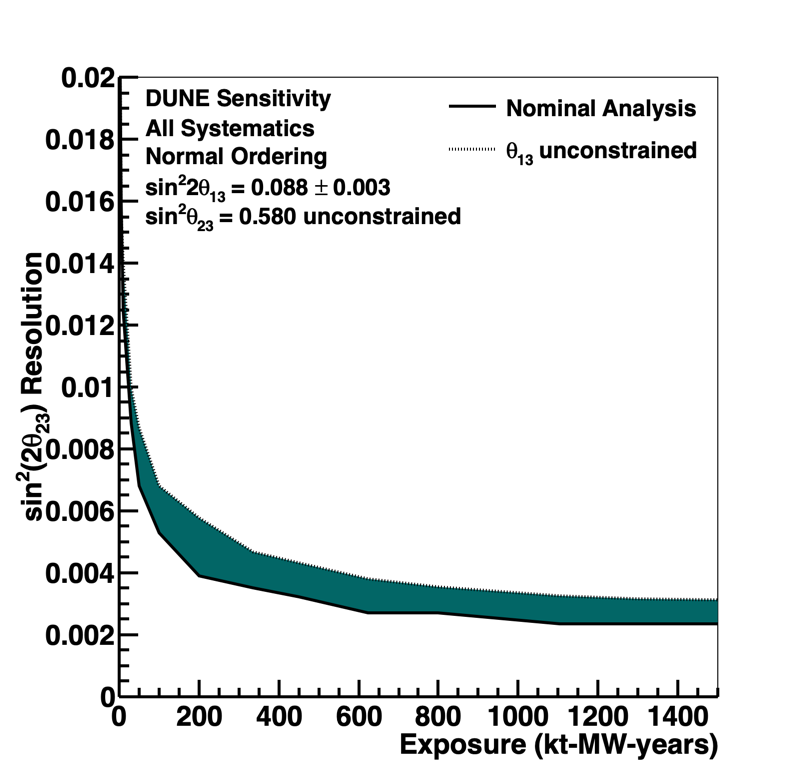
\includegraphics[width=0.475\linewidth]{th23res_exp_varyconstr_nh_2019_v4.png} &
		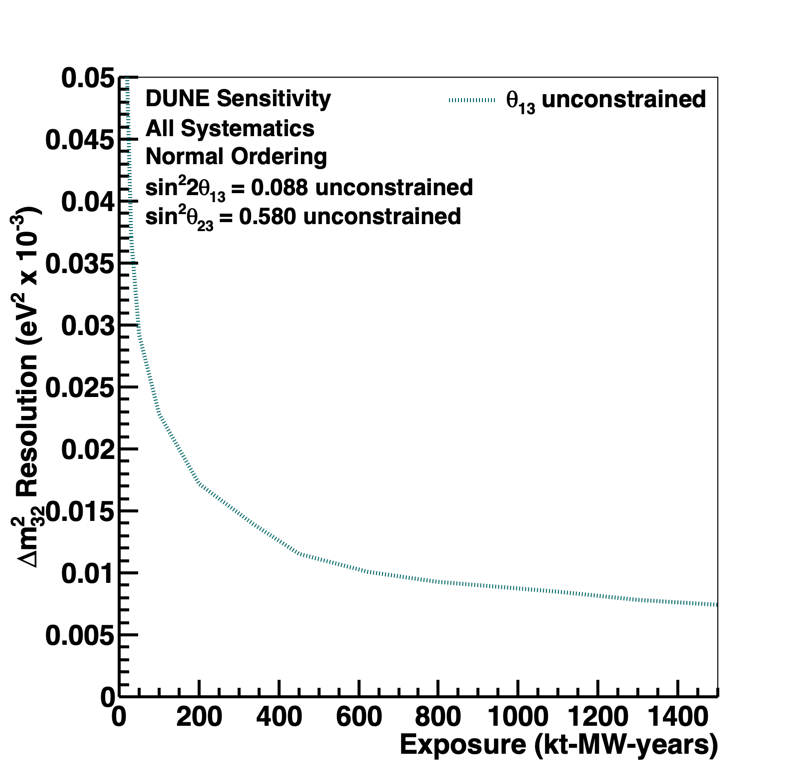
\includegraphics[width=0.475\linewidth]{dmsqres_exp_varyconstr_nh_2019_v4.png} 
	\end{tabular}  
	\caption[Resolution of DUNE measurements of \deltacp and \sinstt{13}, as a function of exposure]{Resolution of DUNE measurements of \sinstt{23} (left) and $\Delta m^{2}_{32}$ (right), as a function of exposure in kt-MW-years. The width of the band for the \sinstt{23} resolution shows the impact of applying an external constraint on \sinstt{13}. For the $\Delta m^{2}_{32}$ resolution, an external constraint does not have a significant impact, so only the unconstrained curve is shown.}
    \label{fig:disres_exp}
\end{figure}

One of the principal strengths of \dword{dune} is its ability to simultaneously measure all oscillation parameters governing long-baseline neutrino oscillation, without a need for external constraints. As an example, Figure~\ref{fig:res_th23vdcp_degen} shows the 90\% C.L.\ allowed regions for \sinst{23} and \deltacp for 7, 10 and 15 years of running, 
compared to the current measurements from world data.
Specifically, it explores the resolution sensitivity that is expected 
for values of \sinst{23} different from the \dword{nufit} central value.  In the plot on the 
left, the value of \sinstt{13} is constrained by external measurements, while on the right no external constraint is applied.
It is interesting to note that the lower-exposure, opposite-octant solutions for \sinst{23} are allowed at 90\% C.L.\ in the absence of an external constraint on \sinstt{13}; however, at the 10 year exposure, this degeneracy is resolved by \dword{dune} data without external constraint.



\begin{figure}[h!]
    \centering
    \begin{tabular}{cc}
		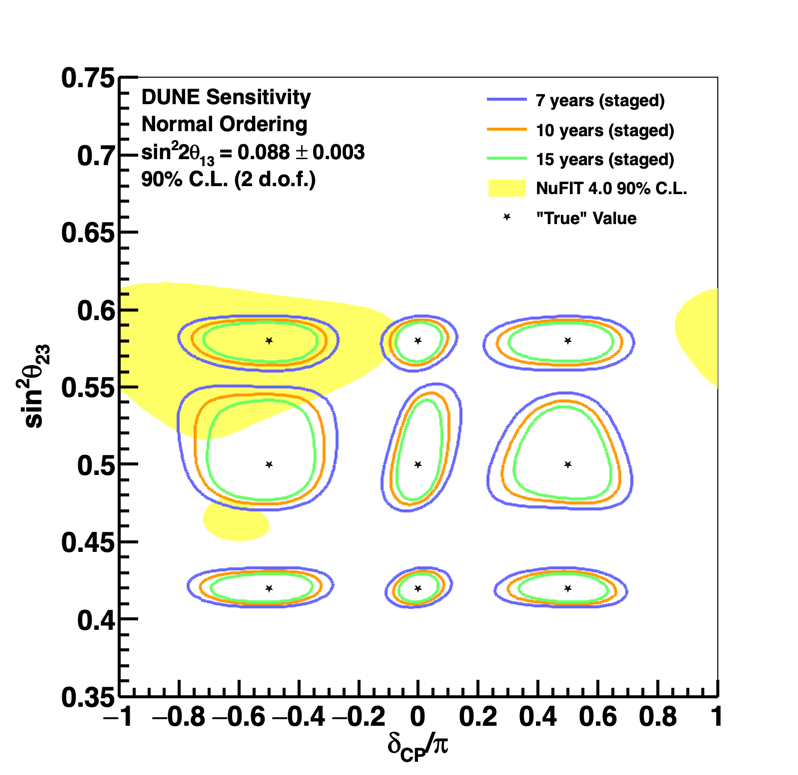
\includegraphics[width=0.475\linewidth]{bubbles_q23_2019_v4.png} &
		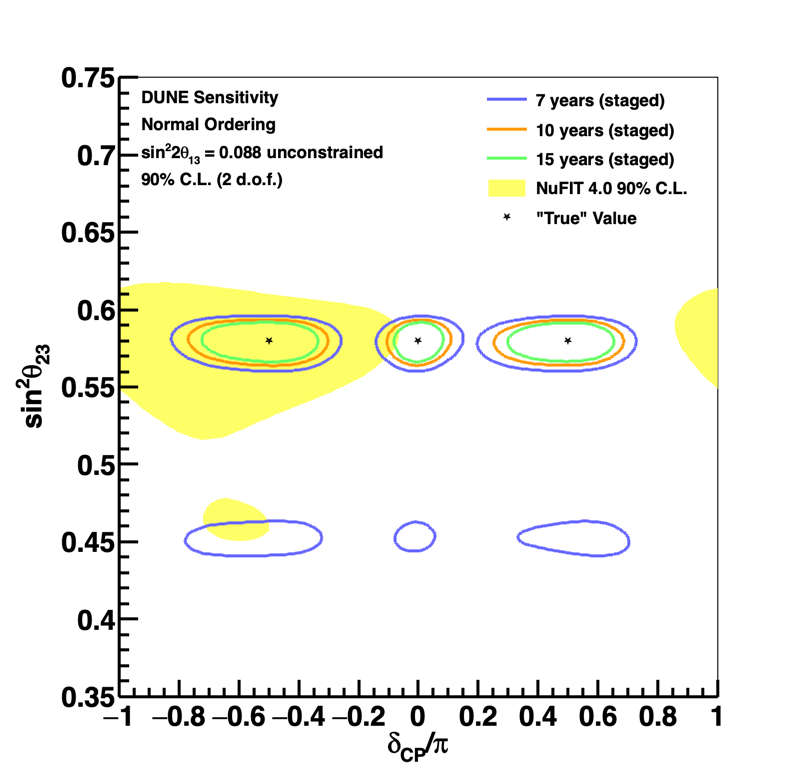
\includegraphics[width=0.475\linewidth]{bubbles_q23_nopen_2019_v4.png} 
	\end{tabular}  
	\caption[Two-dimensional 90\% C.L. region in \sinst{23} and \deltacp]{Two-dimensional 90\% C.L. region in \sinst{23} and \deltacp, for 7, 10, and 15 years of exposure, with equal running in neutrino and antineutrino mode. The 90\% C.L. region for the \dword{nufit} global fit is shown in yellow for comparison. Several possible true values of the oscillation parameters, denoted by stars, are considered, and \sinstt{13} is constrained (left) or unconstrained (right) by \dword{nufit}. In the plot on the right, only one value for \sinst{23} is shown; without the constraint on \sinstt{13}, degenerate regions are allowed for lower exposures.}
    \label{fig:res_th23vdcp_degen}
\end{figure}

The measurement of $\nu_\mu \rightarrow \nu_\mu$ oscillations is sensitive to $\sin ^2 2 \theta_{23}$, whereas the measurement of $\nu_\mu \rightarrow \nu_e$ oscillations is sensitive to $\sin^2 \theta_{23}$.  A combination of both $\nu_e$ appearance and $\nu_\mu$ disappearance measurements can probe both maximal mixing and
the $\theta_{23}$ octant.  
Figure~\ref{fig:lbloctant} shows the sensitivity to determining the octant as a function of the true value of $\sinst{23}$.

\begin{figure}[h!]
    \centering
		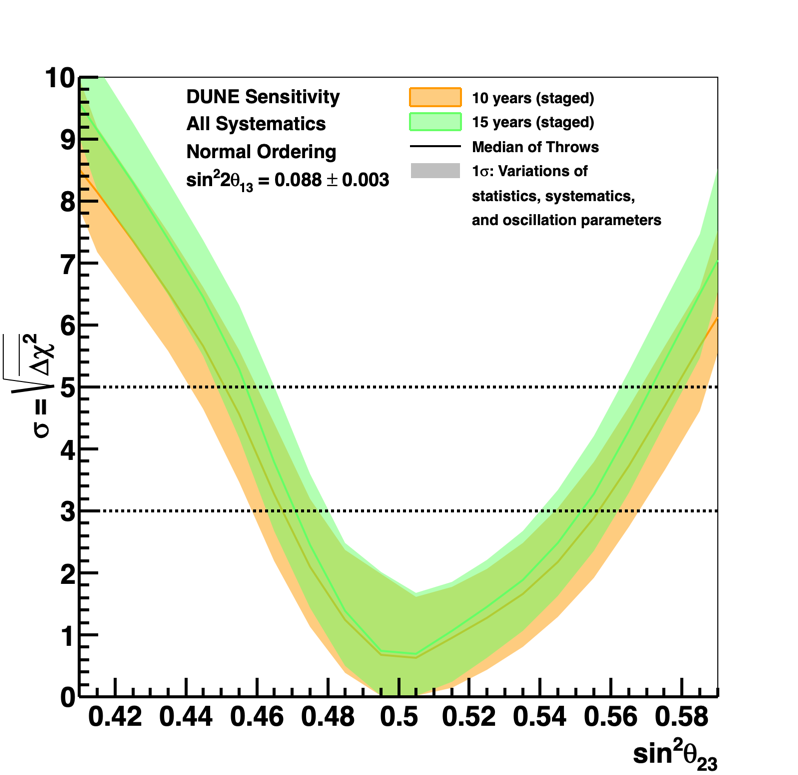
\includegraphics[width=0.5\linewidth]{octant_no_2019_v4.png}
	\caption[Sensitivity of determination of the $\theta_{23}$ octant as a function of \sinst{23}]{Sensitivity to determination of the $\theta_{23}$ octant as a function of the true value of \sinst{23}, for ten (orange) and fifteen (green) years of exposure. True normal ordering is assumed. The width of the transparent bands cover 68\% of fits in which random throws are used to simulate statistical variations and select true values of the oscillation and systematic uncertainty parameters, constrained by pre-fit uncertainties. The solid lines show the median sensitivity.}
    \label{fig:lbloctant}
\end{figure}

\clearpage
%%%%%%%%%%%%%%%%%%%%%%%%%%%%%%%%%%%%%%%%%%%%%%%%%%%%%%%%%%%%%%
\subsection{Proton Decay and Other 
Baryon-number Violating Processes}

By virtue of its deep underground location and large fiducial 
mass, as well as its excellent event imaging, particle 
identification and 
calorimetric capabilities, the \dword{dune} \dword{fd} will be 
a powerful instrument %for discovery of (Anne suggests ``to probe'')
to probe baryon-number violation.
\dword{dune} will be able to observe signatures of decays of protons and 
neutrons, as well as the phenomenon of neutron-antineutron mixing, 
at rates below the limits placed by the current generation of 
experiments.

Many nucleon decay modes are accessible to \dword{dune}.  
As a benchmark, a particularly compelling discovery channel 
is the decay of a proton to a positive kaon and a neutrino, 
\ptoknubar.  In this channel, the kaon and its decay products 
can be imaged, identified, and tested for kinematic consistency 
with the full decay chain, together with precision sufficient to 
reject backgrounds due to atmospheric muon and neutrino 
interactions. 
Preliminary analysis of single-particle beam and cosmic ray tracks 
in the \dword{pdsp} \dword{lartpc} is already demonstrating the particle 
identification capability of \dword{dune}, as illustrated in 
Figure~\ref{fig:pdsp_dedx_execsum}.  
The signature of the kaon track and its observable decay particles is 
sufficiently rich that a credible claim of evidence for 
proton decay could be made on the basis of just 
one or two sufficiently well-imaged events, for the case 
where background sources are expected to contribute much less 
than one event.

\begin{dunefigure}[Reconstructed $dE/dx$ of protons and muons in 
\dshort{pdsp}]{fig:pdsp_dedx_execsum}
{Energy loss of protons (left) and muons (right) in 1-GeV  
running with the \dword{pdsp} \dword{lartpc} at CERN, as a function of 
residual range.  The protons are beam particles identified from 
beamline instrumentation; the muons are reconstructed stopping 
cosmic rays collected concurrently.  
The red curves represent the mean of the 
corresponding expected signature.  Note the difference in 
the vertical scale of the two plots.  The kaon $dE/dx$ curve 
will lie between the two curves shown.}
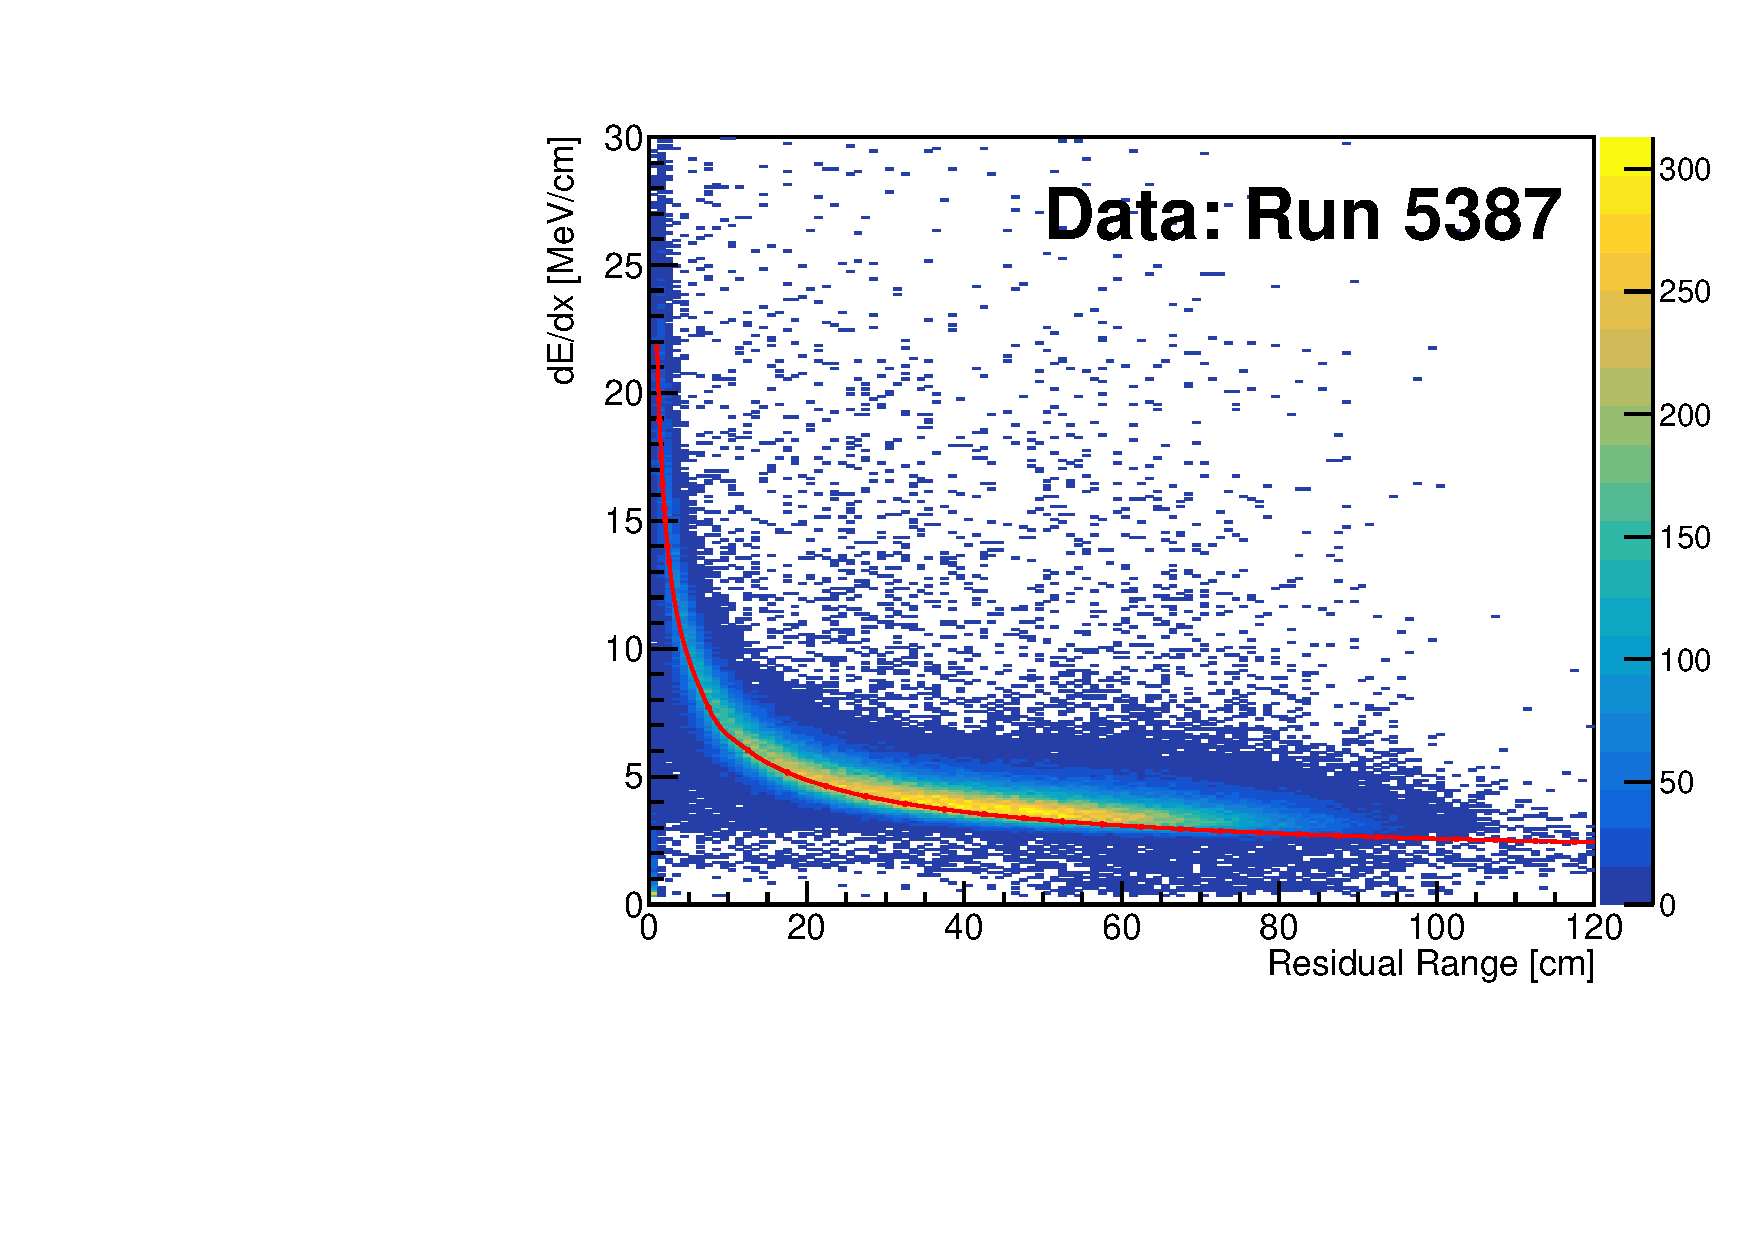
\includegraphics[width=0.45\linewidth]{proton_dedx_resrange_run5387.pdf}\hspace{0.05\linewidth}
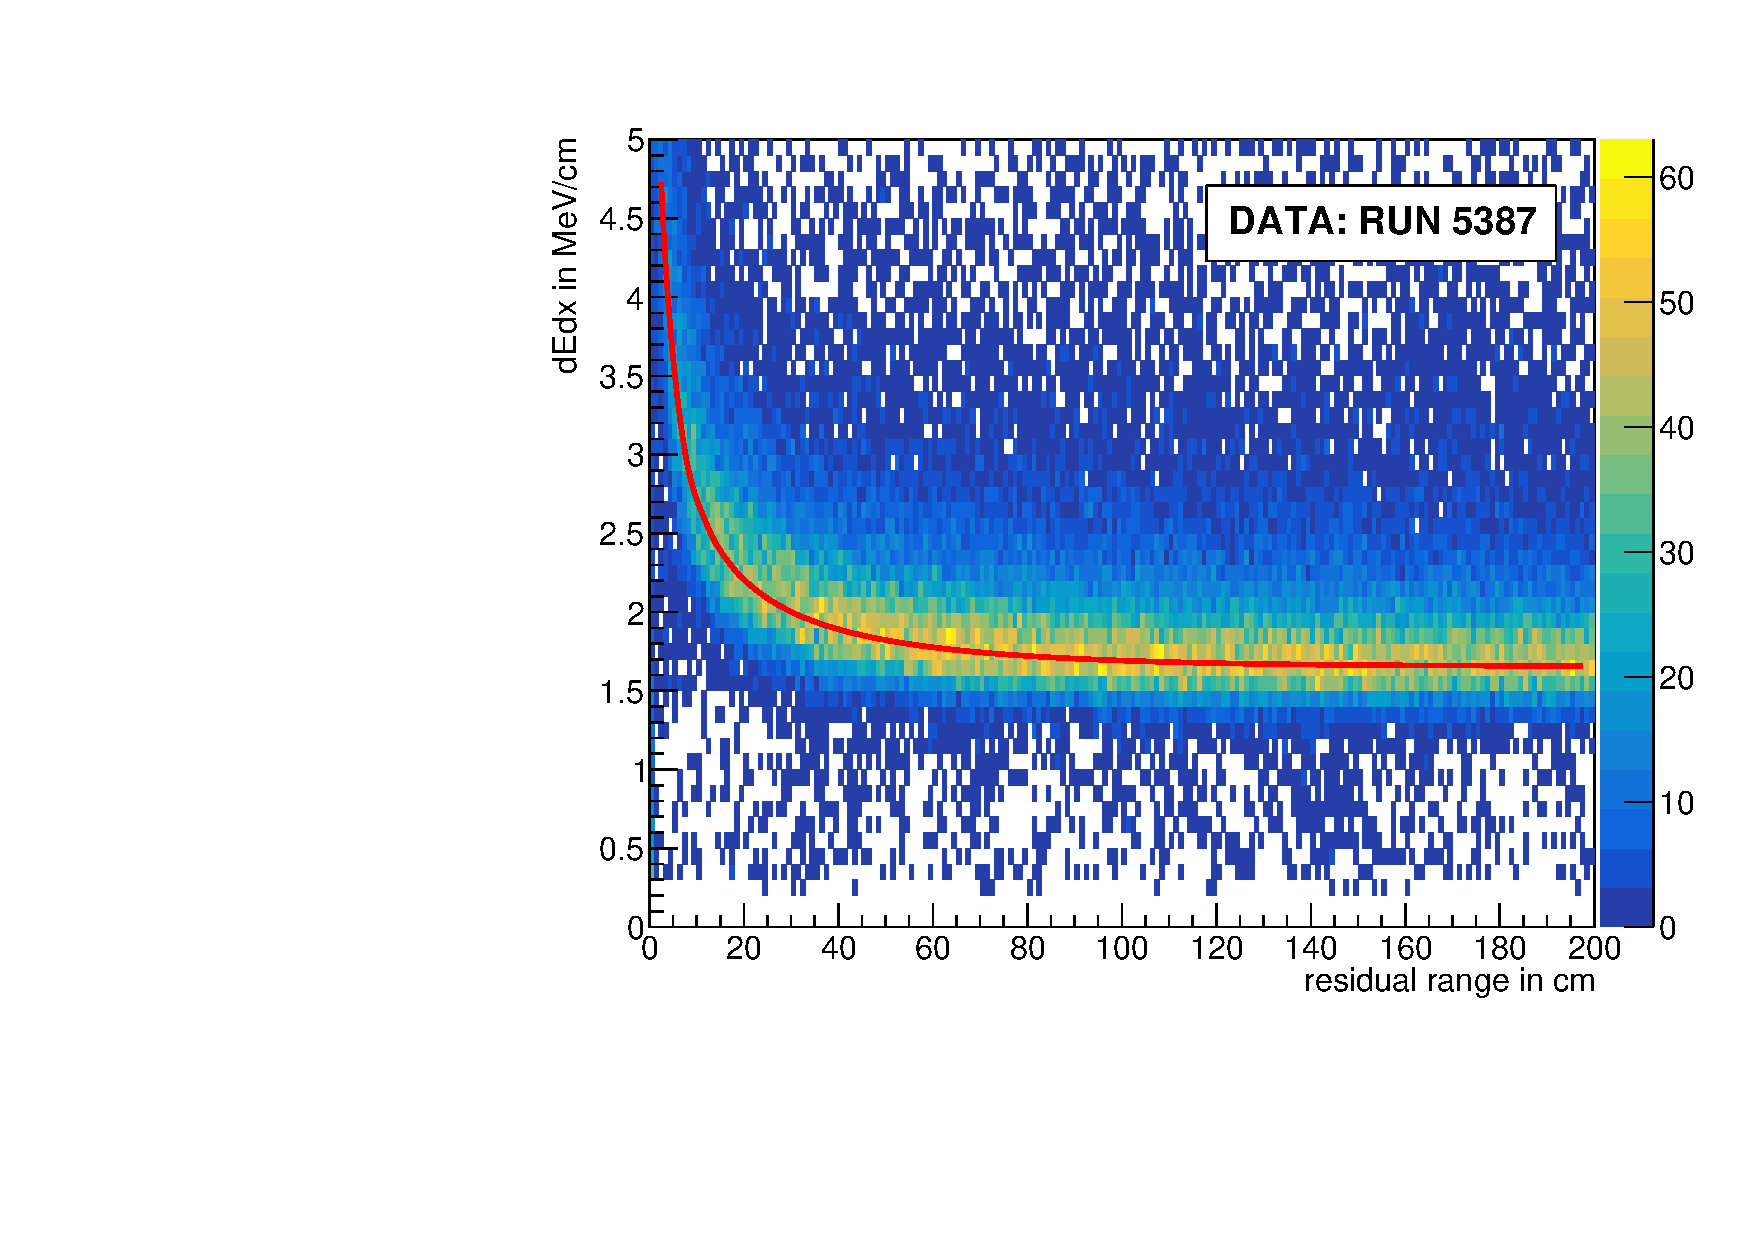
\includegraphics[width=0.45\linewidth]{muon_run5387_dedx.pdf}
\end{dunefigure}

Projecting from the current analysis of \ptoknubar in the \dword{dune} 
\dword{fd}, with a detection efficiency of \num{30}\% as 
described in \physchndk, the 
expected 90\% CL lower limit on lifetime divided by branching 
fraction is \SI{1.3e34}{years} for a 
\num{400}-\SI{}{\ktyr} 
exposure, assuming no candidate events are observed.  This 
is roughly twice the current limit of 
\SI{5.9e33}{years} from \superk~\cite{Abe:2014mwa}, 
based on an exposure of \SI{260}{\ktyr}.  Thus, should the rate 
for this decay be at the current \superk limit, five candidate 
events would be expected in \dword{dune} within ten years 
of running with four \dword{fd} modules.  Ongoing work is aimed 
at improving the efficiency in this and other channels.

%%%%%%%%%%%%%%%%%%%%%%%%%%%%%%%%%%%%%%%%%%%%%%%%%%%%%%%%%%%%%%
\subsection{Galactic Supernovae via Measurements of Neutrino Bursts}
\label{sec:es:phys:galact}

As has been demonstrated with SN1987a, the observation 
of neutrinos~\cite{Bionta:1987qt,Hirata:1987hu} from a 
core-collapse supernova can reveal much about these  
phenomena that is not accessible in its  
electromagnetic signature.  Correspondingly, there is a 
wide range of predictions from supernova models for even 
very basic characteristics of the \dwords{snb}.  Typical  
models predict that a supernova explosion in the 
center of the Milky Way will result in several thousand 
detectable neutrino interactions in the \dword{dune} \dword{fd} 
occurring over an interval of up to a few tens of seconds.
The neutrino energy spectrum peaks around \SI{10}{\MeV}, 
with appreciable flux up to about \SI{30}{\MeV}.

\lar based detectors are sensitive to the \nue 
component of the flux, while water Cherenkov and organic 
scintillator detectors are most sensitive to the \anue 
component.  Thus \dword{dune} is uniquely %well-
positioned to study the 
neutronization burst, in which \nue's are produced during the 
first few tens of milliseconds.  More generally,  
measurements of the (flavor-dependent) neutrino flux and energy 
spectrum as a function of time over the entirety of the burst 
can be sensitive to astrophysical properties of the supernova 
and its progenitor, and distortions relative to nominal 
expectations can serve as signatures for phenomena such 
as shock wave and turbulence effects, or even black hole 
formation.  

Below, we present the results of analyses 
of \dword{dune}'s capabilities for two elements of the \dword{snb} 
 program: (1) fits to the reconstructed 
neutrino energy spectrum and comparison to models in which 
none of the distortions listed above are present, and (2) 
neutrino flux direction determination for angular localization 
of the supernova position.

%%%%%%%%%%%%%%%%%%%%%%%%%%%%%%%%%%%%%%%%%%%%%%%%%%%%%%%%%%%%%%
\subsubsection{Results from Fits to Pinched Thermal Neutrino Energy Spectrum}

The physics of neutrino decoupling and spectra formation is far from trivial, owing to the energy dependence of the cross sections and the roles played by both \dword{cc} and \dword{nc} reactions.
Detailed transport calculations using methods such as \dword{mc} or Boltzmann solvers have been employed. It has been observed that spectra coming out of such simulations can typically be parameterized at a given moment in time by the following ansatz (e.g.,~\cite{Minakata:2008nc,Tamborra:2012ac}):
\begin{equation}
        \label{eq:pinched}
        \phi(E_{\nu}) = \mathcal{N} 
        \left(\frac{E_{\nu}}{\langle E_{\nu} \rangle}\right)^{\alpha} \exp\left[-\left(\alpha + 1\right)\frac{E_{\nu}}{\langle E_{\nu} \rangle}\right] \ ,
\end{equation}
where $E_{\nu}$ is the neutrino energy, $\langle E_\nu \rangle$ is the
mean neutrino energy, $\alpha$ is a ``pinching parameter'', and
$\mathcal{N}$ is a normalization constant that can be related to 
the total binding energy release of the supernova, denoted $\varepsilon$ 
in the discussion below.
%
Large $\alpha$ corresponds to a more ``pinched'' spectrum (suppressed
high-energy tail). This parameterization is referred to as a
``pinched-thermal'' form. The different $\nu_e$, $\overline{\nu}_e$ and
$\nu_x, \, x = \mu, \tau$ flavors are expected to have different
average energy and $\alpha$ parameters and to evolve differently in
time. 

To evaluate \dword{dune}'s capabilities, we have developed a
forward fitting algorithm requiring a binned reconstructed 
neutrino energy spectrum expected for 
a supernova at a given distance generated with a ``true'' set of
pinched-thermal parameters $(\alpha^0, \langle E_\nu \rangle^0,
\varepsilon^0)$.  
Figure~\ref{fig:example3params} shows an example of a resulting fit,
with the approximate parameters for several specific supernova models
superimposed to illustrate the potential for discrimination 
between them.

\begin{dunefigure}[Fit to three supernova neutrino pinched-thermal 
  spectrum parameters]{fig:example3params}{Sensitivity regions for the three
    pinched-thermal parameters (90\% C.L.).
    The simulated data was generated for a supernova at \SI{10}{kpc}
    with a neutrino interaction model appropriate for low energies, 
    realistic detector smearing, and a step efficiency function with a \SI{5}{\MeV}
    detected energy threshold. Superimposed
  are parameters corresponding to the time-integrated flux for three different sets of models:
  Nakazato~\cite{Nakazato:2012qf}, Huedepohl black hole formation models, and Huedepohl
  cooling models~\cite{huedepohldb}.  For the Nakazato parameters (for which there is no
  explicit pinching, corresponding to $\alpha=2.3$), the parameters are
  taken directly from the reference; for the Huedepohl models, they are fit to a
  time-integrated flux.}
	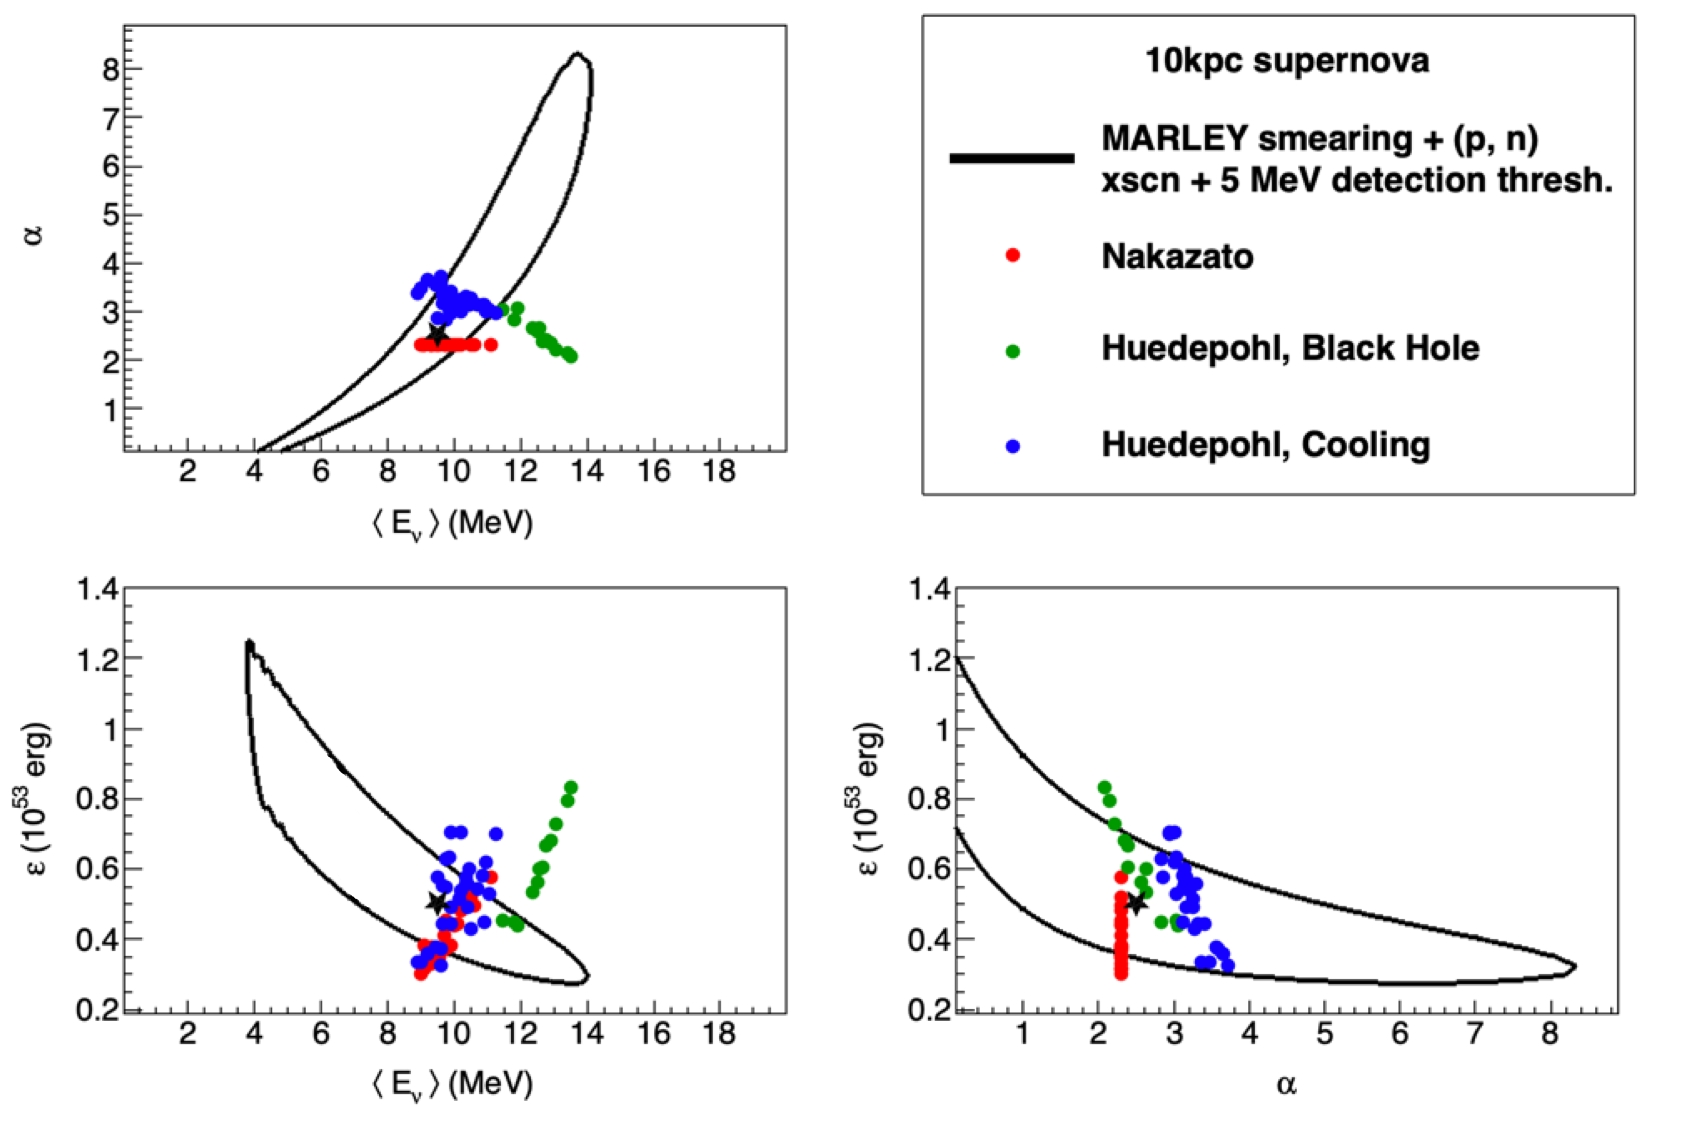
\includegraphics[scale = 0.37]{TDRPlot_Interpolated_ComparingDifferentFluxModels_ExtendedBounds.png}
  \end{dunefigure}

%%%%%%%%%%%%%%%%%%%%%%%%%%%%%%%%%%%%%%%%%%%%%%%%%%%%%%%%%%%%%%
\subsubsection{Pointing Sensitivity of DUNE}

An illustration 
of another element of the \dword{dune} \dword{snb} program 
is given in Figure~\ref{fig:fullSN_execsum}, 
which indicates a pointing resolution of better than $5^\circ$ that 
can be obtained by analysis of both subdominant highly-directional $\nu$-$e$ elastic scattering 
events and dominant weakly-directional $\nu_e$ \dword{cc} events within a \dword{snb}, based 
on full reconstruction and analysis. The \dword{dune} results can be 
combined with corresponding measurements in other neutrino detectors to 
provide supernova localization from neutrinos alone in real time.
%
\begin{dunefigure}[Supernova direction determination from $\nu-e$ elastic scattering events]{fig:fullSN_execsum}{Left: Log
    likelihood values as a function of direction for a
    supernova sample with 260 $\nu$-$e$ elastic scattering (ES) events.  Right: Distribution of angular differences for
    directions to 10-kpc supernova using a maximum likelihood
    method.}
  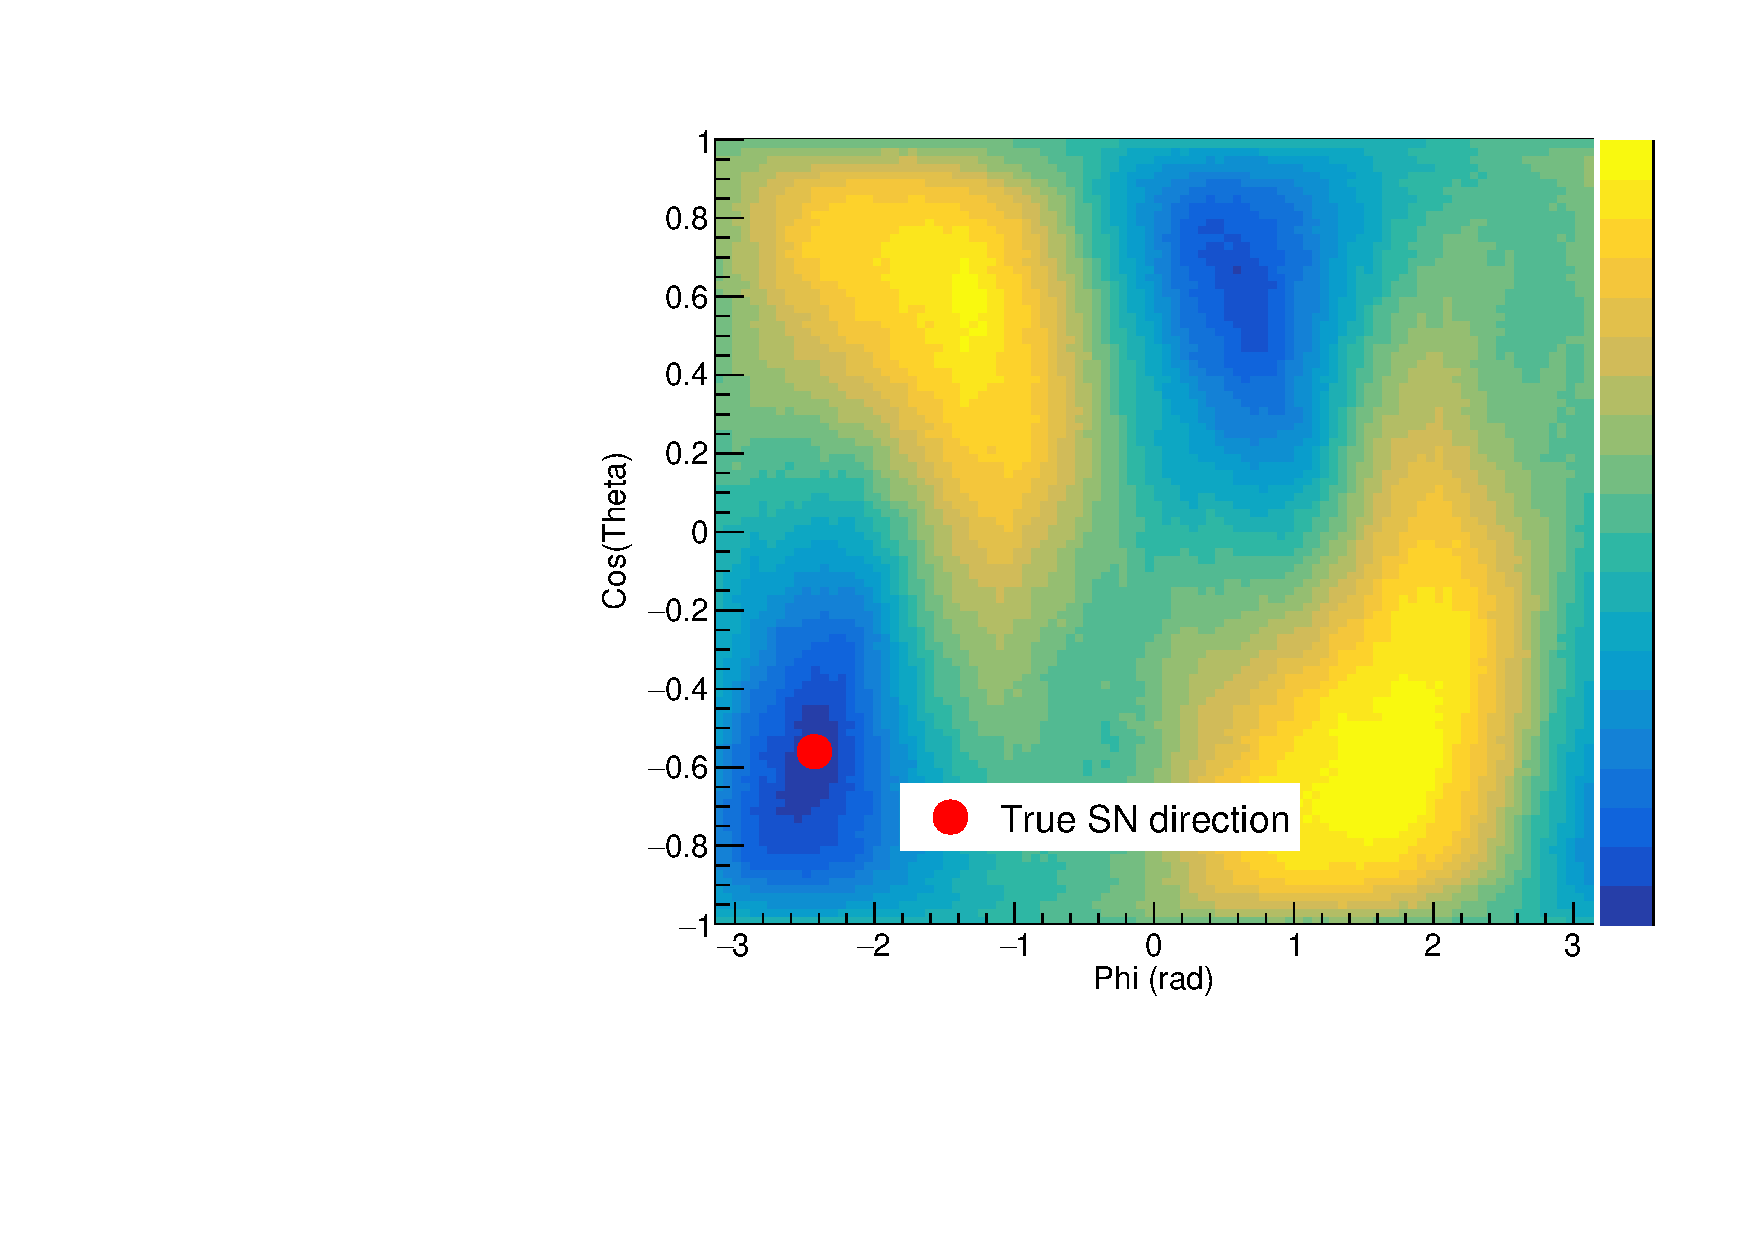
\includegraphics[width=0.44\textwidth]{LLH_252_SNdir.pdf}
  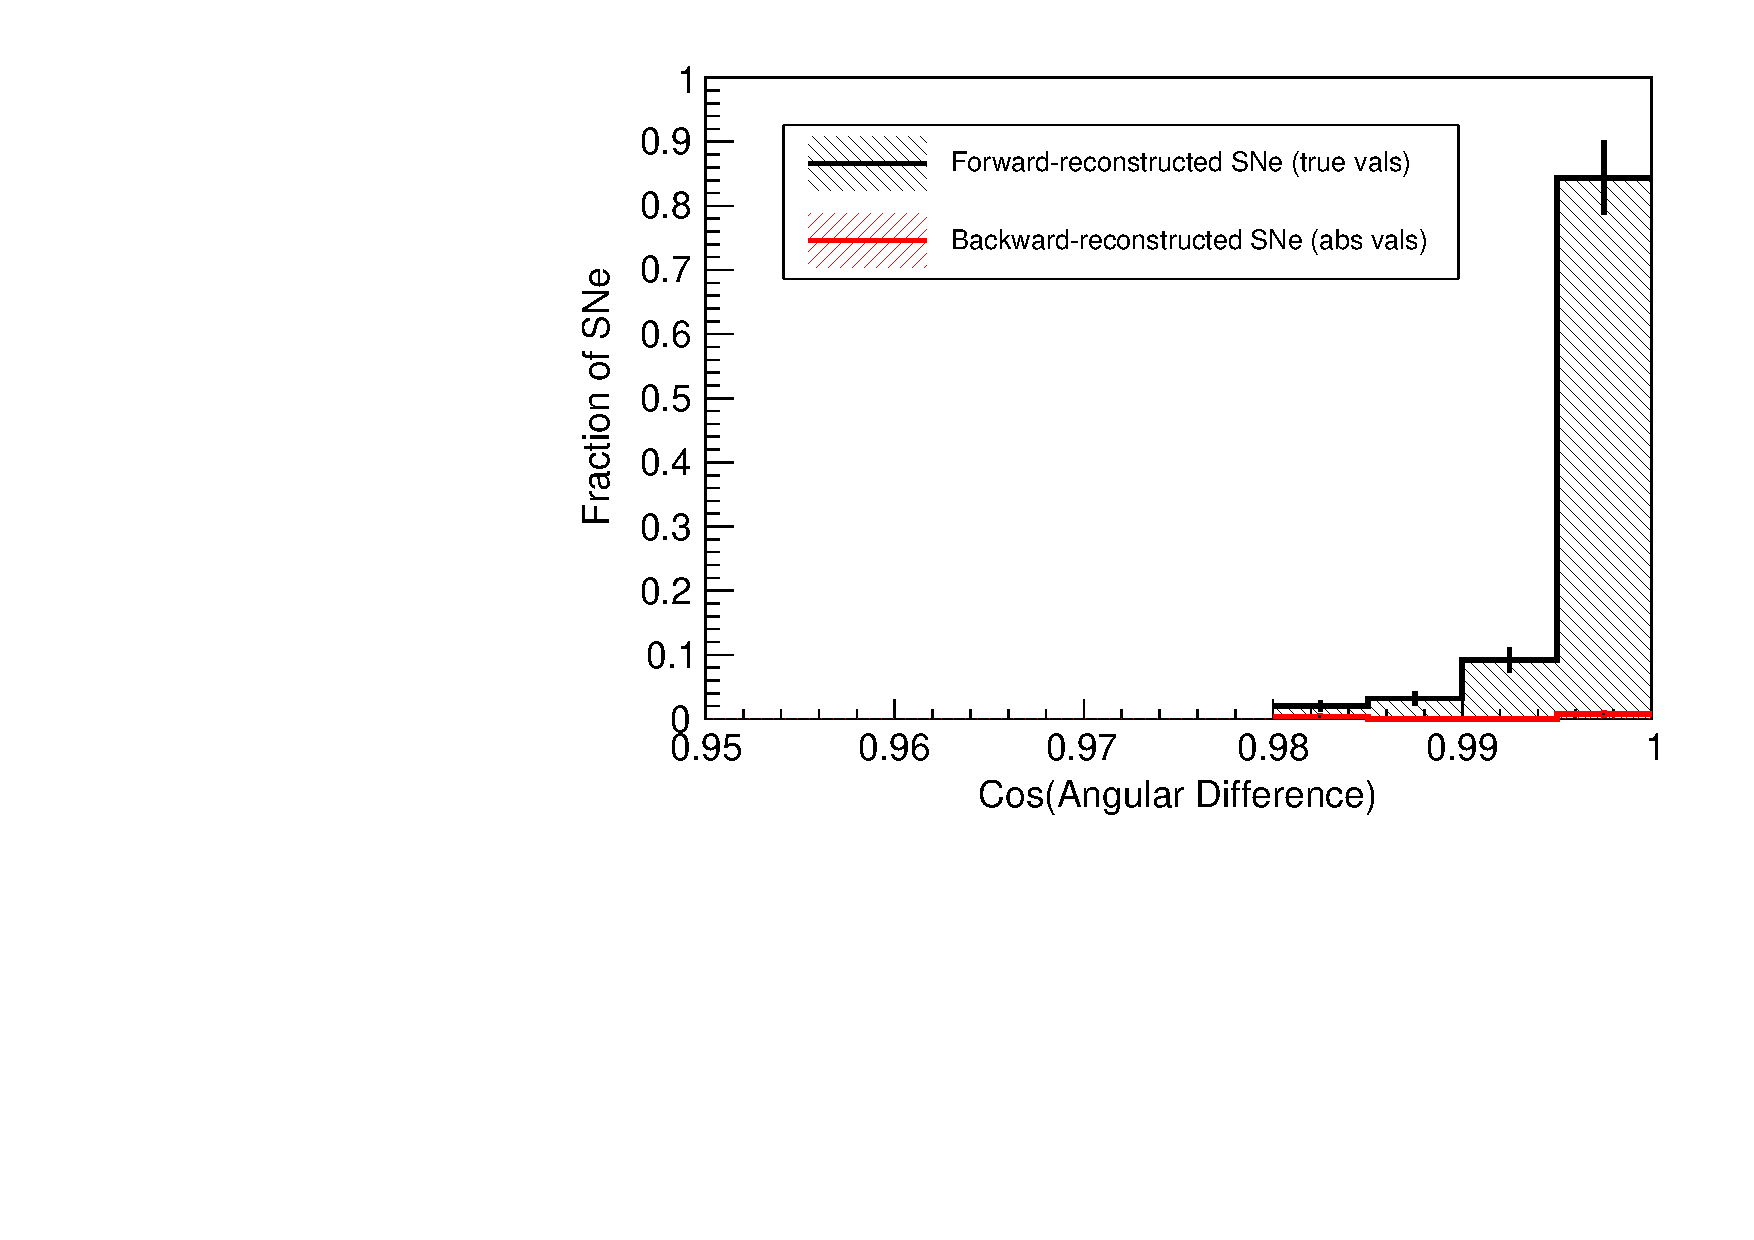
\includegraphics[width=0.48\textwidth]{costheta_fullSN_ESCCPDFs_TDR.pdf}
\end{dunefigure}

%%%%%%%%%%%%%%%%%%%%%%%%%%%%%%%%%%%%%%%%%%%%%%%%%%%%%%%%%%%%%%
\subsection{Searches for Beyond Standard Model Physics}


The unique combination of the high-intensity \dword{lbnf} neutrino beam with
\dword{dune}'s \dword{nd}  and massive \dword{lartpc} \dword{fd} modules at a 
\SI{1300}{\km} baseline enables a variety of probes of \dword{bsm} 
physics, either novel or with unprecedented sensitivity.

As examples of the potential impact of \dword{dune}, we present results from the 
analysis of simulated data sets for two \dword{bsm} scenarios, one with 
a sterile neutrino species participating in oscillations, 
and the other with anomalous ``neutrino trident'' events.
%with di-lepton production 
%generated by a new gauge boson mediating neutrino interaction 
%in the Coulomb field of a nucleus that accompanies the lepton 
%outgoing from the neutrino vertex.
%
From the sterile neutrino analysis,  
the \dword{dune} sensitivities to the effective mixing angle $\theta_{\mu e}$
(which depends on new mixing angles $\theta_{14}$ and $\theta_{24}$), from the appearance and disappearance samples at the \dword{nd} and \dword{fd} are shown in Figure~\ref{fig:th_me2}. 
%

Considering a neutrino trident analysis in \dword{nd} data, 
existing constraints and projected sensitivity to parameters of a $Z^\prime$ boson resulting from the gauging of the difference between 
muon and tau lepton numbers, $L_\mu - L_\tau$, are presented 
in Figure~\ref{fig:LmuLtau2}.  This plot indicates that \dword{dune} 
can cover much of parameter space for which this model is 
able to explain the 
departure of the present observed muon $g-2$ central value 
from standard model expectations.


\begin{dunefigure}
[Sensitivity to effective mixing angle $\theta_{\mu e}$ from 
a DUNE sterile neutrino analysis]
{fig:th_me2}
{DUNE 90\% CL sensitivities to $\theta_{\mu e}$ from the appearance and disappearance samples at the \dword{nd} and \dword{fd} is shown along with a comparison with previous existing experiments and the sensitivity from the future \dword{sbn} program. Regions to the right of the DUNE contours are excluded.}
$\vcenter{\hbox{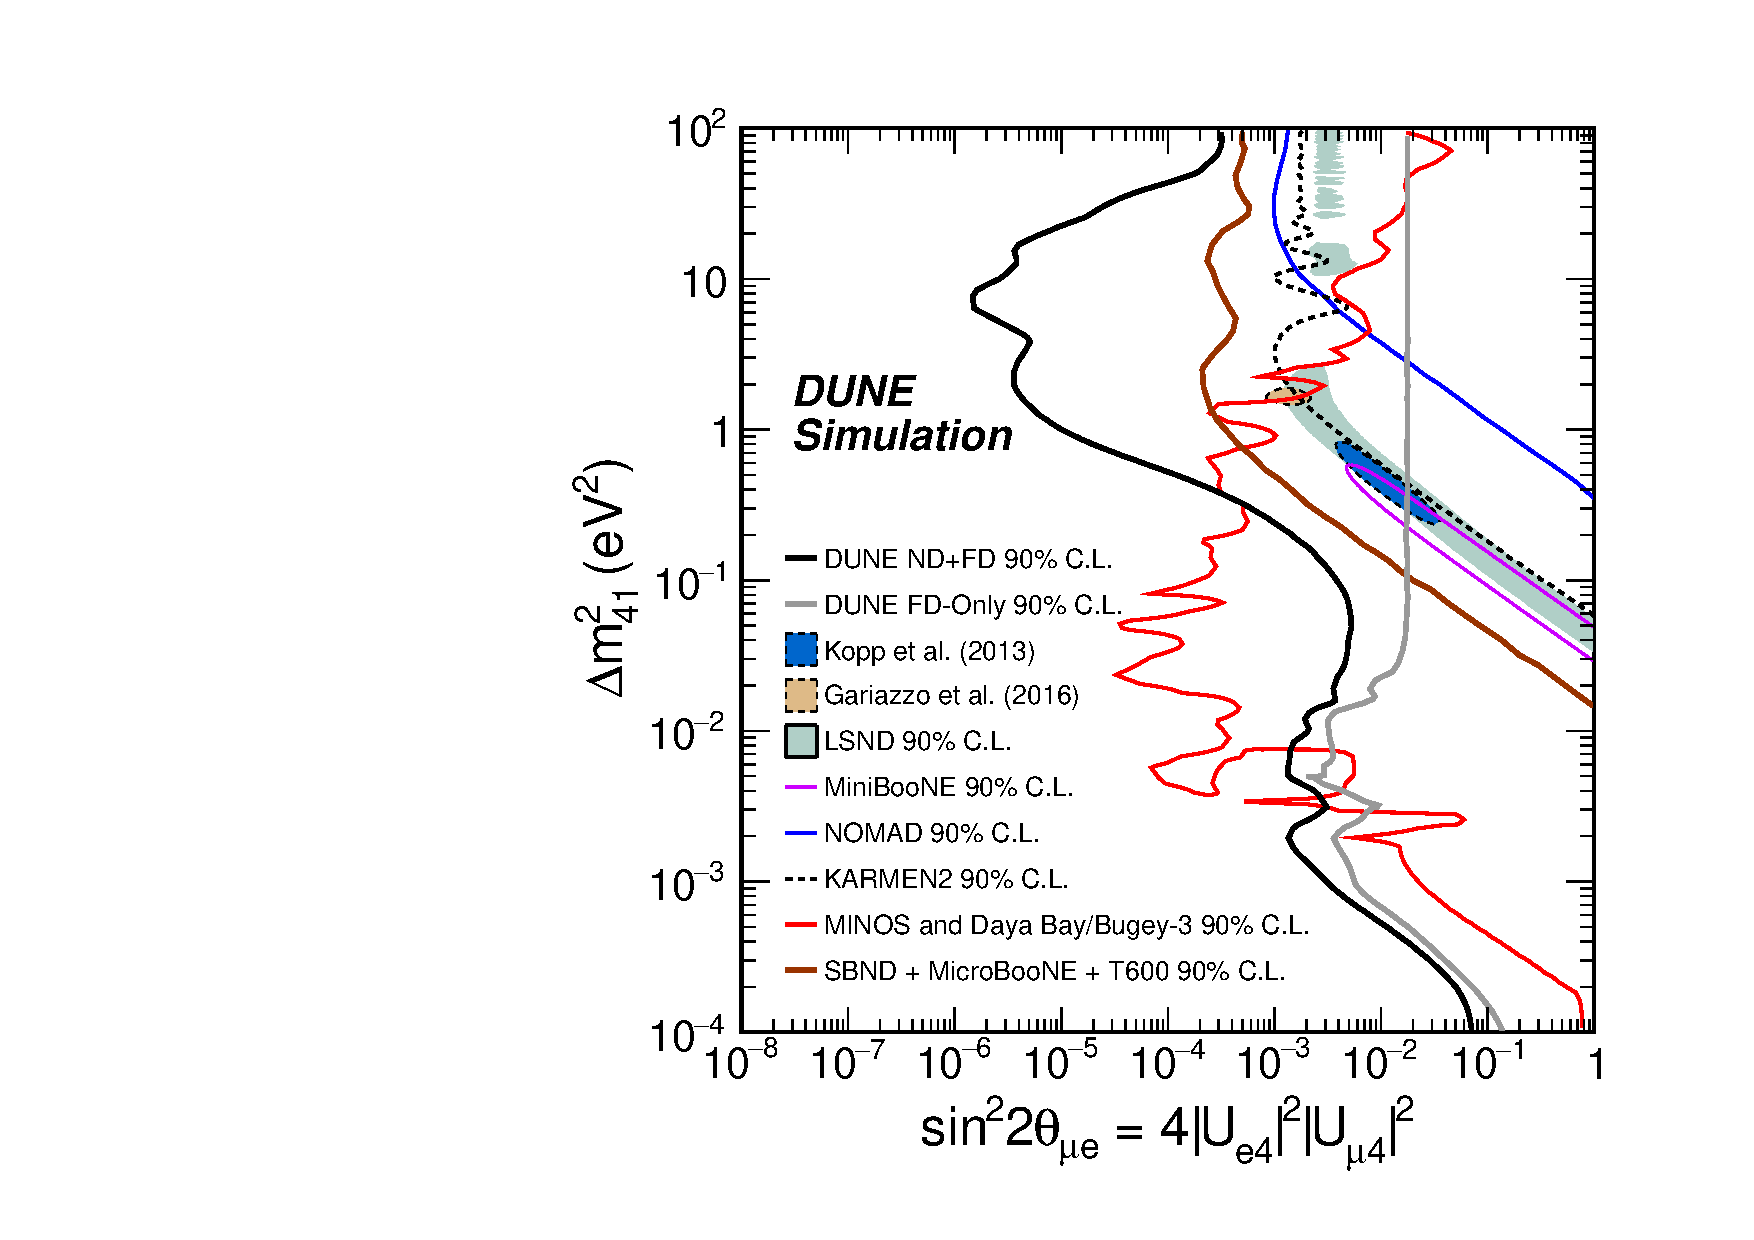
\includegraphics[width=0.70\columnwidth]{ComboLimit90_dune_sbn.pdf}}}$
\end{dunefigure}

\begin{figure}[tb!] \centering
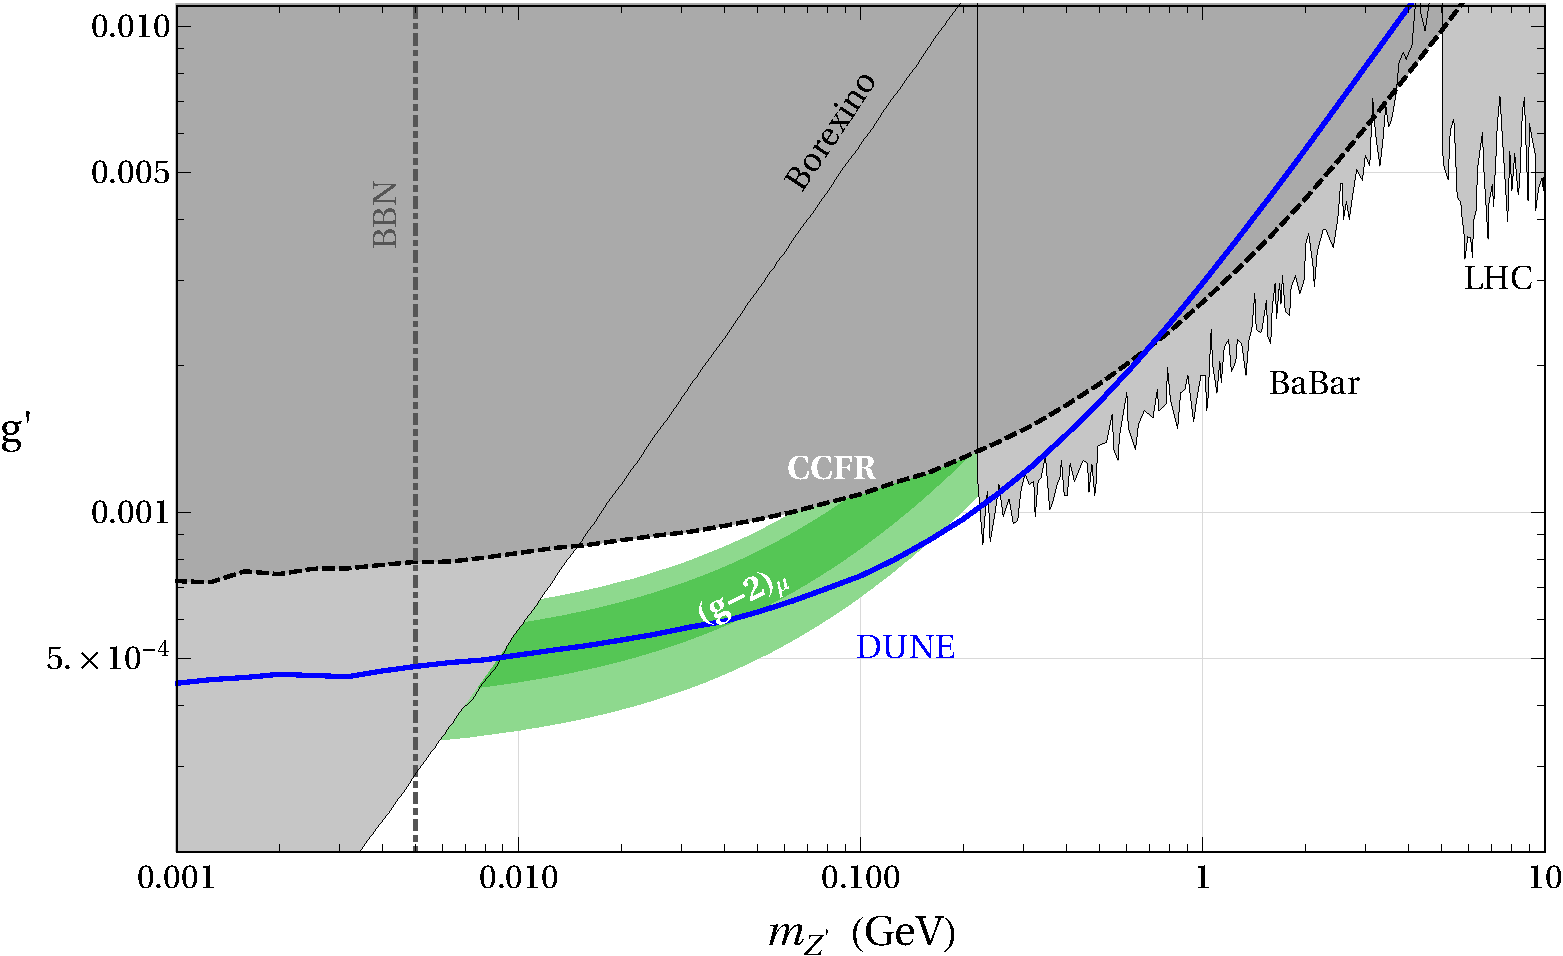
\includegraphics[width=0.75\textwidth]{LmuLtau_zoom.pdf}
\caption[Projected sensitivity to BSM 
contributions to neutrino trident events]{Existing constraints and projected \dword{dune} sensitivity in the $Z^\prime$ parameter spaced associated with gauging $L_\mu - L_\tau$. Shown in green is the region where the $(g-2)_\mu$ anomaly can be explained at the $2\sigma$ level. The parameter regions already excluded by existing constraints are shaded in gray and correspond to a CMS search for $pp \to \mu^+\mu^- Z' \to \mu^+\mu^-\mu^+\mu^-$~\cite{Sirunyan:2018nnz} (``LHC''), a BaBar search for $e^+e^- \to \mu^+\mu^- Z' \to \mu^+\mu^-\mu^+\mu^-$~\cite{TheBABAR:2016rlg} (``BaBar''), precision measurements of $Z \to \ell^+ \ell^-$ and $Z \to \nu\bar\nu$ couplings~\cite{ALEPH:2005ab,Altmannshofer:2014cfa} (``LEP''), a previous measurement of the trident cross section~\cite{Mishra:1991bv,Altmannshofer:2014pba} (``CCFR''), a measurement of the scattering rate of solar neutrinos on electrons~\cite{Bellini:2011rx,Harnik:2012ni,Agostini:2017ixy} (``Borexino''), and bounds from Big Bang Nucleosynthesis~\cite{Ahlgren:2013wba,Kamada:2015era} (``BBN''). The \dword{dune} sensitivity shown by the solid blue line assumes a measurement of the trident cross section with $40\%$ precision.}
\label{fig:LmuLtau2}
\end{figure}
